% =====================================================================
%  Articulo COMPLETO - Observatorio de Participación de Graduados USTA 2026-1
%  Hallazgos del cruce: SECOP, RUES y CvLAC, con vision por seccionales
%  Secciones redactadas por subagentes -> _build_cruce/sec_*.tex
%  Compilar: pdflatex (MiKTeX) dos veces.
% =====================================================================
\documentclass[11pt,letterpaper]{article}
\usepackage[utf8]{inputenc}
\usepackage[T1]{fontenc}
\usepackage[spanish,es-noquoting]{babel}
\usepackage[letterpaper,margin=2.3cm,top=2.6cm,bottom=2.4cm]{geometry}
\usepackage{lmodern}
\usepackage{graphicx}
\usepackage{float}
\usepackage{xcolor}
\usepackage{colortbl}
\usepackage{booktabs}
\usepackage{array}
\usepackage{tabularx}
\usepackage{enumitem}
\usepackage{fancyhdr}
\usepackage{titlesec}
\usepackage{abstract}
\usepackage[most]{tcolorbox}
\usepackage{siunitx}
\sisetup{group-separator={.}, group-minimum-digits=4, output-decimal-marker={,}, detect-weight=true, detect-family=true}
\usepackage{csquotes}
\usepackage[hidelinks]{hyperref}

\definecolor{ustaazul}{HTML}{1F3A93}
\definecolor{ustadorado}{HTML}{E8A317}
\definecolor{ustarojo}{HTML}{B22222}
\definecolor{ustagris}{HTML}{444444}
\definecolor{ustagrisclaro}{HTML}{F2F4F8}
\definecolor{ustacrema}{HTML}{FBF3DC}
\definecolor{ustaverde}{HTML}{1B998B}
\definecolor{ustaborde}{HTML}{D5DAE3}

\pagestyle{fancy}
\fancyhf{}
\renewcommand{\headrulewidth}{0.4pt}
\renewcommand{\footrulewidth}{0.4pt}
\fancyhead[L]{\footnotesize\color{ustagris}Observatorio de Participación de Graduados}
\fancyhead[R]{\footnotesize\color{ustagris}Consultorio de Estadística $\cdot$ 2026-1}
\fancyfoot[C]{\footnotesize\color{ustagris}\thepage}

\titleformat{\section}{\large\bfseries\color{ustaazul}}{\thesection.}{0.5em}{}
\titleformat{\subsection}{\normalsize\bfseries\color{ustarojo}}{\thesubsection}{0.5em}{}
\titlespacing*{\section}{0pt}{12pt}{5pt}
\titlespacing*{\subsection}{0pt}{8pt}{3pt}

\setlist[itemize]{leftmargin=1.3em, itemsep=1.5pt, topsep=2pt}
\renewcommand{\labelitemi}{\textcolor{ustadorado}{\textbullet}}
\newcolumntype{L}[1]{>{\raggedright\arraybackslash}p{#1}}
\newcommand{\code}[1]{\texttt{\small #1}}

\newtcolorbox{cajaobs}{colback=ustacrema, colframe=ustadorado, boxrule=1pt,
  borderline west={3pt}{0pt}{ustarojo}, arc=2pt, left=10pt, right=8pt, top=8pt, bottom=8pt}
\newtcolorbox{cajahallazgo}{colback=ustagrisclaro, colframe=ustaazul, boxrule=1pt,
  borderline west={3pt}{0pt}{ustaverde}, arc=2pt, left=10pt, right=8pt, top=8pt, bottom=8pt}

\begin{document}

\begin{center}
  
\includegraphics[width=2.4cm]{UstaLogo.png}\\[4pt]
  {\footnotesize\color{ustagris} Universidad Santo Tomás $\cdot$ Facultad de Estadística\\
  Consultorio de Estadística $\cdot$ Organización \texttt{ustadistica}}\\[10pt]
  {\LARGE\bfseries\color{ustaazul} Observatorio de Participación de Graduados}\\[4pt]
  {\large\color{ustarojo} Trayectoria de los graduados de la USTA en SECOP, RUES y CvLAC,\\ con análisis por seccional}\\[3pt]
  {\normalsize\itshape Informe de hallazgos --- Periodo 2026-1 (fase de integración y análisis)}\\[10pt]
  {\normalsize\bfseries Consultorio de Estadística}\\[3pt]
  {\footnotesize\color{ustagris} Sobre la base de fuentes recolectada y catalogada por Natalia González, Ximena Arias y Paula Gordillo\\
  Repositorio de referencia: \href{https://github.com/ustadistica/impacto_graduados}{\code{ustadistica/impacto\_graduados}}}
\end{center}
\vspace{4pt}\hrule height 0.8pt\vspace{8pt}

\begin{abstract}
\noindent El informe anterior del \emph{Observatorio de Participación de Graduados} concluyó que el trabajo de 2026-1 recolectó y catalogó con solvencia tres fuentes oficiales ---CvLAC/GrupLAC, RUES y SNIES--- pero que el \textbf{cruce integrado} entre ellas, razón de ser del observatorio, había quedado pendiente. Este artículo retoma ese punto y reporta, con análisis descriptivo, comparación por sedes y cruce de variables, los hallazgos de \textbf{ejecutar el cruce}. Sobre una base unificada de \textbf{174.685 graduados} de la Universidad Santo Tomás (seis sedes: Sede Principal de Bogotá, Bucaramanga, Tunja, Villavicencio, Medellín y los centros VUAD de educación a distancia; 1970--2026), se enlazó a cada egresado ---por documento de identidad--- con el \textbf{SECOP Integrado} (contratación pública) y el \textbf{RUES} (registro mercantil), y ---por evidencia académica--- con \textbf{CvLAC} (investigación). Los resultados perfilan por primera vez de forma integrada la huella del egresado: el \textbf{24,6\,\%} aparece como proveedor del Estado, el \textbf{21,5\,\%} ha registrado empresa y un grupo selecto figura como investigador con vínculo USTA comprobado. En conjunto, \textbf{el 40,3\,\% deja huella en al menos una de las tres dimensiones} y un núcleo de \textbf{227 personas} lo hace en las tres. El análisis por sedes revela patrones contrastantes ---Tunja lidera en contratación pública e investigación, Bucaramanga en matrícula mercantil, y Bogotá figura entre las tasas más bajas pese a su enorme volumen--- y un fuerte arraigo territorial: cada sede contrata y se registra en el RUES sobre todo en su propio departamento. El cruce de variables muestra, además, que los investigadores contratan y se registran en el RUES muy por encima del promedio. El cruce que el observatorio tenía pendiente es, hoy, su primer mapa de la participación del egresado. \\[4pt]
\noindent\textbf{Palabras clave:} egresados, participación, cruce de fuentes, resolución de identidades, seccionales, SECOP, RUES, CvLAC, datos abiertos, API Socrata.
\end{abstract}
\vspace{2pt}

\section{Introducción}

Medir la participación de un egresado es, paradójicamente, más difícil cuanto más valioso resulta esa participación. La universidad acompaña al estudiante con un detalle minucioso a lo largo de su formación —cada materia, cada nota, cada semestre queda registrado—, pero pierde de vista al graduado justo en el momento en que comienza lo que mejor refleja el valor de aquello que aprendió: su inserción en el mercado laboral, la creación de una empresa, la producción de conocimiento científico. La trayectoria que más importa para juzgar la pertinencia de un programa es, precisamente, la que ocurre fuera de los muros de la institución y, por tanto, fuera de sus sistemas de información.

El obstáculo no es solo de seguimiento, sino de observación. Ninguna fuente única alcanza a mirar al egresado en todas sus facetas. El registro de contratación pública sabe quién firma contratos con el Estado, pero ignora quién montó un negocio o quién publica artículos. El registro mercantil conoce al matriculado en el RUES, pero no al investigador ni al contratista. La plataforma de ciencia y tecnología documenta al académico, pero permanece ciega ante la vida empresarial o la prestación de servicios al sector público. Cada registro nacional es una ventana parcial: nítida en su dominio, muda en los demás. De ahí nace el valor de \emph{cruzar}: solo al superponer esas ventanas parciales aparece una figura completa del graduado, y solo entonces puede afirmarse —con evidencia y no con encuestas— qué hace la USTA con quienes forma.

\subsection{El punto de partida heredado}

Este artículo no parte de cero. Continúa, con respeto y con espíritu autocrítico, el trabajo del equipo que nos precedió (Natalia González, Ximena Arias y Paula Gordillo), cuyo informe dejó una conclusión tan honesta como incómoda. Aquel equipo recolectó y catalogó con rigor las fuentes que alimentarían el observatorio —CvLAC y GrupLAC de Minciencias, el RUES de las cámaras de comercio y el SNIES del Ministerio de Educación— y describió bien cada una por separado. Sin embargo, reconoció que faltaba lo esencial: no existió un identificador que enlazara a un mismo egresado entre fuentes distintas. Sin ese puente, el cruce —que es la razón de ser misma de un observatorio de participación— quedó pendiente. El informe lo expresó sin eufemismos: el observatorio había quedado \enquote{en fase de cimientos}.

Tomamos esa frase como punto de partida y no como reproche. Unos buenos cimientos son condición necesaria para levantar un edificio; lo que faltaba era levantarlo. La pregunta que organiza este artículo es directa: ¿qué se ve cuando, por fin, las fuentes se cruzan entre sí?

\subsection{Qué cambia en esta fase}

Tres decisiones metodológicas separan esta fase de la anterior. La primera es trabajar sobre un universo concreto de graduados de la USTA, no sobre muestras ni aproximaciones. La integración de un padrón institucional ampliado triplicó la base de análisis: ahora son 174.685 graduados con títulos otorgados entre 1970 y 2026, distribuidos en seis sedes encabezadas por la Sede Principal de Bogotá y acompañadas por Bucaramanga, Tunja, Villavicencio, Medellín y la modalidad a distancia de la VUAD. Cada persona que figura en ese padrón es buscada, una por una, en los registros nacionales.

La segunda decisión es resolver el enlace por documento contra el universo completo de cada registro —no contra un extracto—, y hacerlo del lado del servidor, de modo que la coincidencia se establezca sobre el identificador único de la persona y no sobre atributos frágiles. Así se cruza a los 174.685 egresados contra la totalidad de SECOP y del RUES, evitando las pérdidas y los falsos positivos propios de los cotejos manuales o por aproximación de nombres.

La tercera atiende el caso particular de CvLAC, donde el documento de identidad no está disponible. Allí la coincidencia por nombre sería peligrosamente endeble, de manera que sustituimos esa coincidencia por una validación basada en evidencia académica —la formación declarada y la pertenencia a grupos de investigación—, exigiendo respaldo verificable antes de dar por enlazada a una persona. El resultado es un cruce que ya no descansa sobre suposiciones, sino sobre identificadores y evidencia.

\subsection{Panorama de hallazgos}

El alcance del ejercicio puede resumirse en pocas cifras macro. El universo analizado comprende 174.685 graduados de la USTA, con títulos otorgados entre 1970 y 2026, distribuidos en las seis sedes ya mencionadas. Al cruzar ese universo contra los tres registros, encontramos que el 40,3\% de los graduados —70.377 personas— deja huella verificable en al menos una de las tres dimensiones de participación consideradas. Dicho de otro modo, cerca de cuatro de cada diez egresados santotomasinos aparece, hoy y de forma rastreable, como contratista del Estado, como matriculado en el RUES formal o como investigador reconocido.

Por dimensión, las tasas globales dibujan un perfil claro. La contratación pública (SECOP) es la huella más extendida, con cerca del 24\% de los graduados registrados como proveedores del Estado: 42.889 personas. La matrícula mercantil formal (RUES) alcanza alrededor del 21,5\%, con 37.544 matriculados en el RUES. La investigación (CvLAC), por su naturaleza más selectiva y por el criterio estricto de validación que aplicamos, identifica a un grupo reducido pero cualitativamente significativo de 2.547 graduados. En el extremo más exigente del cruce —la intersección de las tres dimensiones a la vez— encontramos a 227 personas que son, simultáneamente, contratistas, empresarias e investigadoras: un núcleo pequeño de egresados de participación múltiple que solo se vuelve visible cuando las fuentes se miran juntas.

\begin{cajahallazgo}
El cruce que el observatorio tenía pendiente —su deuda declarada, su \enquote{fase de cimientos}— es hoy su primer hallazgo. Al enlazar a los 174.685 graduados de la USTA contra SECOP, RUES y CvLAC, comprobamos que más de un tercio de los egresados (40,3\%) deja una huella pública y verificable de su participación profesional, empresarial o científica. El observatorio dejó de ser una promesa de datos bien guardados para convertirse en una afirmación con evidencia.
\end{cajahallazgo}

El resto del artículo recorre este hallazgo de lo general a lo particular. Primero caracterizamos al universo de graduados por sede, programa y cohorte, para saber de quiénes hablamos. Luego examinamos cada dimensión por separado —la huella en contratación pública, el tejido matriculado en el RUES y el perfil investigador—, atendiendo a su magnitud, su composición y sus matices. A continuación abordamos el cruce integrado: cómo se combinan las dimensiones, dónde se solapan y qué perfiles de participación múltiple emergen. Después proyectamos los resultados sobre el territorio, y cerramos con una discusión que interpreta los hallazgos, reconoce los límites del enlace y traza las siguientes obras sobre los cimientos ya levantados.

\section{Datos y método}

El trabajo previo del equipo —Natalia González, Ximena Arias y Paula Gordillo— dejó planteada una tensión que esta sección busca resolver de manera operativa: caracterizar la participación de los graduados de la Universidad Santo Tomás exige confrontar nuestros propios registros institucionales con fuentes nacionales heterogéneas, cada una con su lógica de identificación, su escala y sus límites de acceso. El método que describimos a continuación no parte de un universo descargado y luego filtrado, sino de la pregunta inversa: a quién, de entre nuestros graduados, encuentran las fuentes externas. Esa inversión es la que hace viable —y reproducible— el cruce.

\subsection{Base unificada de graduados}

El primer requisito fue construir una sola base de graduados a partir de cuatro insumos institucionales que hasta ahora vivían por separado. El insumo central es la base SPB-CM-CAU, que reúne la Sede Principal de Bogotá, el Campus Medellín y los centros VUAD de educación a distancia; a este se suman la base de Bucaramanga, la de la Seccional Tunja y la de la Seccional Villavicencio. Cada insumo se proyectó sobre un esquema común, conservando una columna de procedencia que garantiza la \emph{trazabilidad de la fuente}: en todo momento es posible saber de cuál de las bases proviene cada registro, condición indispensable para los análisis por sede que sostienen el resto del artículo.

La integración produjo \textbf{197.273} registros de grado asociados a \textbf{174.685} documentos únicos, con una cobertura temporal que va de \textbf{1970} a \textbf{2026}. La diferencia entre ambas cifras no es ruido: refleja que una misma persona puede figurar con más de un grado (por ejemplo, pregrado y posgrado, o dos posgrados, eventualmente en sedes distintas), de modo que el registro es la unidad documental y el documento es la unidad poblacional sobre la que se mide la participación.

La incorporación de la base SPB-CM-CAU resuelve la principal limitación de la fase anterior, en la que la Sede Principal de Bogotá no estaba presente. Con su integración, el universo de análisis cubre las seis sedes de la Universidad y queda representado en la totalidad de los cruces posteriores, de manera que la participación de los egresados bogotanos deja de ser una ampliación pendiente y pasa a formar parte del alcance de este informe.

Dos normalizaciones fueron decisivas para que el enlace posterior no fracasara por motivos formales. La primera recae sobre la identificación: cada documento se reduce a \emph{solo dígitos}, eliminando puntos, espacios, guiones y prefijos, de manera que una misma cédula escrita de distintas maneras en distintas bases converja a una única clave de cruce. La segunda recae sobre los nombres de programa, homogeneizados para que variantes ortográficas o de mayúsculas no fragmenten un mismo programa en categorías espurias. La Tabla~\ref{tab:base_unificada} resume el aporte de cada sede, distinguiendo el total de registros incorporados de los graduados efectivamente consolidados en la base unificada.

\begin{table}[htbp]
\centering
\caption{Composición de la base unificada de graduados por sede.}
\label{tab:base_unificada}
\begin{tabularx}{\linewidth}{Xrr}
\toprule
\rowcolor{ustaazul}
\textbf{\color{white}Sede} & \textbf{\color{white}Registros} & \textbf{\color{white}Graduados} \\
\midrule
Bogotá & 115.473 & 104.468 \\
Bucaramanga & 40.989 & 37.370 \\
Tunja & 17.925 & 14.859 \\
Villavicencio & 7.619 & 7.030 \\
Medellín & 3.634 & 3.374 \\
VUAD & 11.633 & 11.098 \\
\midrule
\textbf{Total (suma por sede)} & \textbf{197.273} & \textbf{178.199} \\
\textbf{Total (personas únicas)} & & \textbf{174.685} \\
\bottomrule
\end{tabularx}
\\[3pt]{\footnotesize\color{ustagris} La suma de graduados por sede (178.199) supera el total de personas únicas (174.685) porque 3.514 personas obtuvieron títulos en más de una sede y se contabilizan en cada una. La unidad poblacional del resto del informe es la persona única.}
\end{table}

\subsection{Enlace por documento contra registros nacionales (SECOP y RUES)}

Las dos fuentes que identifican a las personas por número de documento —el Sistema Electrónico de Contratación Pública y el Registro Único Empresarial y Social— se publican como conjuntos de datos abiertos en plataformas Socrata, lo que abre una vía de enlace que evita por completo descargar el universo. La clave está en resolver el cruce \emph{del lado del servidor}: en lugar de traer los datos a casa y filtrarlos, se le pide a la API que sea ella quien filtre.

Concretamente, se emplea el lenguaje de consulta SoQL para enviar peticiones por lotes con la forma \code{documento IN (lista\_de\_cédulas)}, agrupadas por documento. La API recibe un subconjunto de nuestras cédulas, busca las coincidencias dentro del registro nacional y devuelve únicamente los resultados agregados por persona; el resto del universo nunca viaja por la red. Esta arquitectura es la que vuelve tratable un problema que, abordado por fuerza bruta, sería prohibitivo: el SECOP Integrado (\code{rpmr-utcd}) contiene del orden de 22 millones de contratos y el RUES (\code{c82u-588k}) cerca de 9,3 millones de matrículas mercantiles. De manera complementaria, se recuperó el clasificador UNSPSC del objeto contractual desde SECOP II (\code{jbjy-vk9h}), que describe la naturaleza de los bienes y servicios contratados. Descargar y cruzar localmente esos volúmenes carecería de sentido cuando lo que nos interesa es, apenas, la intersección con \textbf{174.685} cédulas.

La eficiencia del enfoque es notable. Las 174.685 cédulas se despachan por lotes y cada fuente completa su barrido sin almacenamiento intermedio del universo ni costos de transferencia desproporcionados. El resultado es un cruce que puede repetirse a voluntad —por ejemplo, cuando se actualicen los registros nacionales— con un costo computacional marginal.

\subsection{Validación por evidencia académica (CvLAC)}

La tercera fuente, el CvLAC de Minciencias, obliga a cambiar de estrategia porque no comparte la lógica de las dos anteriores. El CvLAC no publica el número de documento ni admite búsqueda por cédula: cada hoja de vida se identifica mediante un código interno, el \code{cod\_rh}. En consecuencia, el único punto de contacto inmediato con nuestra base es el nombre, y el cruce por nombre es, por construcción, ambiguo —homónimos, abreviaturas y variantes hacen que una coincidencia de cadena no constituya, por sí sola, prueba de identidad ni de vínculo institucional.

Para no contaminar el análisis con falsos positivos, se exigió \emph{evidencia} de vínculo con la Universidad Santo Tomás antes de aceptar cualquier coincidencia. Esa evidencia adopta dos formas, no excluyentes: la aparición de la Universidad Santo Tomás en la formación académica declarada en el perfil, y la pertenencia a un grupo de investigación USTA según GrupLAC, donde el enlace es exacto porque el integrante queda asociado a su \code{cod\_rh}. Cada coincidencia recibe finalmente un \emph{score} en una escala de 0 a 100, que pondera la fuerza de la evidencia y permite separar enlaces sólidos de meras aproximaciones nominales.

\begin{cajaobs}
La cobertura de las tres fuentes es asimétrica y debe leerse en consecuencia. SECOP y RUES se enlazan por documento sobre la totalidad de los graduados, de modo que sus tasas son comparables y casi exhaustivas. El CvLAC, en cambio, se valida por evidencia y sobre un subconjunto necesariamente parcial: la ausencia de búsqueda por cédula y la exigencia probatoria implican que una persona con producción académica real puede no aparecer si no media evidencia explícita de su vínculo USTA. Las cifras de las tres dimensiones, por tanto, no deben leerse en pie de igualdad.
\end{cajaobs}

\section{Caracterización de los graduados por sede}

La integración de las bases del Observatorio reúne a 174.685 graduados de la Universidad Santo Tomás repartidos en sus seis sedes. El análisis que sigue describe el tamaño relativo de cada una, su trayectoria temporal, los programas que definen su perfil y la composición de su oferta entre pregrado y posgrado, para cerrar con una síntesis comparativa que contrasta el volumen con la participación agregada.

\subsection{Tamaño y peso de cada sede}

La distribución de graduados está fuertemente concentrada en la Sede Principal de Bogotá, que reúne 104.468 personas, es decir, alrededor de seis de cada diez graduados de toda la Universidad. A considerable distancia aparece Bucaramanga con 37.370 graduados, seguida por Tunja con 14.859 y la VUAD con 11.098. Las seccionales de Villavicencio y Medellín, con 7.030 y 3.374 graduados respectivamente, completan el conjunto como las de menor tamaño.

El número de registros académicos supera siempre al de personas, porque un mismo graduado puede haber obtenido más de un título en la Universidad. Esa brecha es más amplia precisamente donde la oferta de posgrados es más densa: en Bogotá los 115.473 registros frente a 104.468 personas reflejan una proporción apreciable de graduados que regresaron para cursar una especialización o una maestría, y en Tunja los 17.925 registros frente a 14.859 personas apuntan en el mismo sentido. En las sedes más jóvenes o de menor tamaño la diferencia entre registros y personas se estrecha, señal de que la formación posgradual todavía no ha generado allí la misma circulación de egresados.

\begin{figure}[H]\centering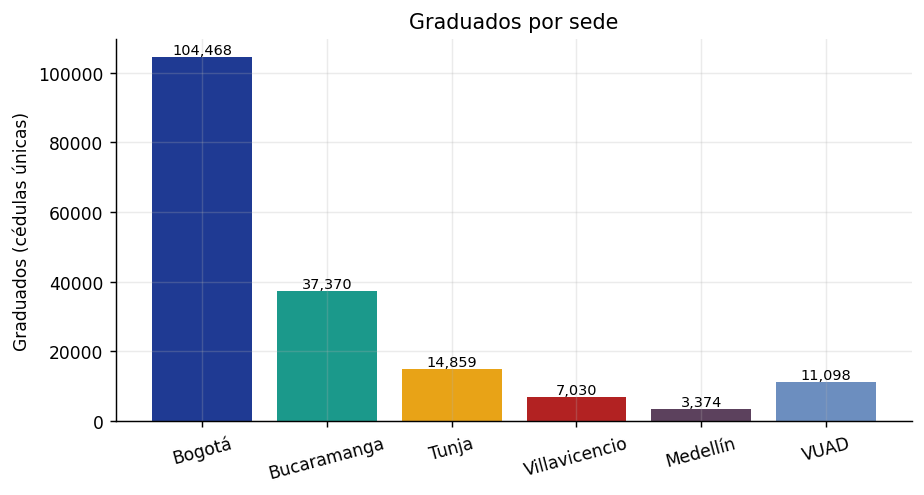
\includegraphics[width=0.82\linewidth]{figs_cruce/01_grad_seccional.png}\caption{Graduados por sede seccional. Bogotá concentra cerca del 60\% del total.}\label{fig:gradsec}\end{figure}

La Figura~\ref{fig:gradsec} hace visible el contraste de escalas: la Sede Principal no solo encabeza el conjunto, sino que multiplica varias veces el tamaño de cualquier seccional, lo que condiciona buena parte de las cifras agregadas que se presentan más adelante.

\subsection{Evolución histórica}

La cobertura temporal de la base se extiende entre 1970 y 2026. La Sede Principal de Bogotá aporta la serie más larga y voluminosa, con graduaciones que se remontan al inicio del periodo y un máximo histórico de 6.225 títulos en 1999, una cifra que ninguna otra sede se acerca a igualar. Las seccionales presentan trayectorias más recientes y picos de magnitud mucho menor: Bucaramanga alcanza su máximo en 2025 con 2.024 graduados, Tunja también en 2025 con 1.620, Villavicencio en 2024 con 921, la VUAD en 2018 con 902 y Medellín en 2023 con 238.

El arranque tardío de Villavicencio, cuyo pico se sitúa apenas en 2024, ilustra cómo varias seccionales se consolidaron como centros de graduación en fechas relativamente recientes, mientras Bogotá ya acumulaba décadas de egresados. El año 2026 se excluye de la lectura de tendencias por corresponder a un periodo todavía en curso, cuyos registros están incompletos.

\begin{figure}[H]\centering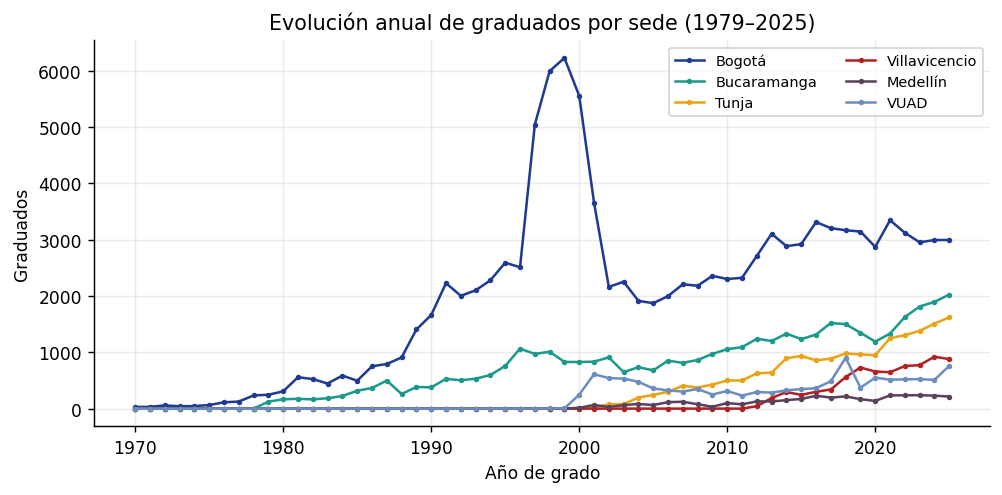
\includegraphics[width=0.82\linewidth]{figs_cruce/02_evolucion_seccional.png}\caption{Evolución anual de graduaciones por sede, 1970--2025.}\label{fig:evolucion}\end{figure}

La Figura~\ref{fig:evolucion} muestra estas trayectorias superpuestas y deja ver tanto el predominio sostenido de Bogotá como la incorporación escalonada de las demás sedes a lo largo de las últimas décadas.

\subsection{Programas dominantes}

El perfil formativo de la Universidad se define por un núcleo de programas de las ciencias jurídicas, económicas y administrativas. Derecho encabeza con holgura la lista, con 19.086 graduados, seguido por Contaduría Pública con 10.254. A continuación aparecen la Especialización en Derecho Administrativo con 8.887, Negocios Internacionales con 7.867 y Economía con 7.107, lo que confirma el peso de la formación posgradual jurídica dentro de la oferta.

Las ingenierías y la arquitectura ocupan un lugar destacado, con Ingeniería Civil (6.574) y Arquitectura (6.019) entre los diez programas más numerosos, acompañadas más abajo por Ingeniería Electrónica. La presencia de Administración de Empresas (6.085), Psicología (5.004) y Odontología (3.964) amplía el espectro hacia las ciencias sociales y de la salud. Las licenciaturas, vinculadas en buena medida a la educación a distancia, completan el cuadro con programas en educación preescolar, educación básica y filosofía y ciencias religiosas, que reflejan la vocación humanista y pedagógica de la institución.

\begin{figure}[H]\centering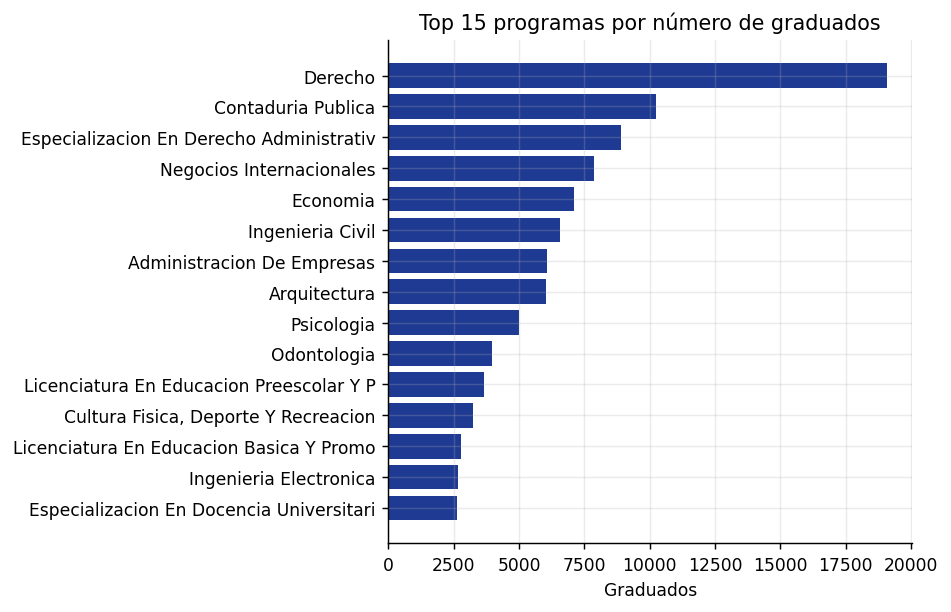
\includegraphics[width=0.82\linewidth]{figs_cruce/03_top_programas.png}\caption{Programas con mayor número de graduados en el conjunto de la Universidad.}\label{fig:topprog}\end{figure}

La Figura~\ref{fig:topprog} ordena estos programas según su volumen de graduados y permite apreciar el dominio de Derecho frente al resto de la oferta.

\subsection{Modalidad de formación}

La composición entre pregrado y posgrado, ahora disponible para las seis sedes, varía de manera notable. Bogotá combina 68.083 graduados de pregrado con 47.390 de posgrado, una proporción posgradual cercana al 41\% que da cuenta de una oferta madura de especializaciones y maestrías. Tunja presenta el perfil más orientado al posgrado, con 7.747 títulos posgraduales frente a 10.178 de pregrado, alrededor del 43\% del total. Bucaramanga, que ahora también reporta modalidad, suma 29.207 graduados de pregrado y 11.782 de posgrado, una proporción posgradual próxima al 29\%.

En el extremo opuesto, Villavicencio y la VUAD concentran su actividad en el pregrado: la primera reporta 5.893 graduados de pregrado frente a 1.726 de posgrado, y la VUAD, ligada a la educación a distancia, suma 9.129 títulos de pregrado por apenas 2.504 de posgrado, en ambos casos alrededor de un 22\% o 23\% posgradual. Medellín ocupa una posición intermedia, con 2.347 graduados de pregrado y 1.287 de posgrado, un peso del posgrado próximo al 35\%.

\begin{figure}[H]\centering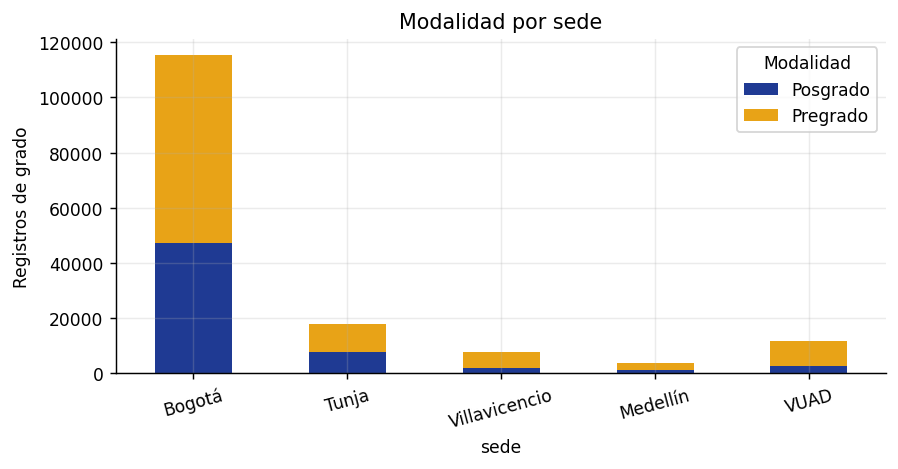
\includegraphics[width=0.82\linewidth]{figs_cruce/04_modalidad_seccional.png}\caption{Distribución de graduados entre pregrado y posgrado por sede.}\label{fig:modalidad}\end{figure}

La Figura~\ref{fig:modalidad} sintetiza estos contrastes y evidencia que la madurez posgradual está asociada a las sedes de mayor trayectoria, como Bogotá y Tunja.

\subsection{Síntesis comparativa por sede}

\begin{table}[H]\centering\scriptsize
\caption{Síntesis comparativa por sede: tamaño, formación y participación.}
\label{tab:seccional_sintesis}
\begin{tabular}{lrrrrrr}
\toprule
\rowcolor{ustaazul}\textbf{\color{white}Indicador} & \textbf{\color{white}Bogotá} & \textbf{\color{white}Bucaramanga} & \textbf{\color{white}Tunja} & \textbf{\color{white}Villavicencio} & \textbf{\color{white}Medellín} & \textbf{\color{white}VUAD} \\
\midrule
Graduados (personas) & 104.468 & 37.370 & 14.859 & 7.030 & 3.374 & 11.098 \\
Posgrado (\% títulos) & 41\% & 29\% & 43\% & 23\% & 35\% & 22\% \\
Programa principal & Derecho & Derecho & Derecho & Derecho & Arquitectura & Administracion D \\
Proveedor (SECOP) & 20,0\% & 28,2\% & 45,2\% & 38,0\% & 28,9\% & 19,9\% \\
Matriculado en RUES & 18,2\% & 29,0\% & 24,8\% & 24,2\% & 17,8\% & 23,3\% \\
Investigador (CvLAC) & 1,5\% & 1,3\% & 2,5\% & 1,2\% & 1,1\% & 0,6\% \\
Con $\geq$1 dimensión & 34,4\% & 49,1\% & 58,0\% & 52,2\% & 40,5\% & 36,4\% \\
\bottomrule
\end{tabular}
\\[2pt]{\scriptsize\color{ustagris} VUAD agrupa los centros de atención universitaria (educación a distancia).}
\end{table}

La tabla anterior reúne en un mismo cuadro el tamaño, la composición formativa y las tasas de participación de cada sede, y revela que el volumen de graduados no determina por sí solo la huella que dejan en el ámbito público, empresarial e investigativo. Tunja lidera la participación agregada: el 45,2\% de sus graduados figura como proveedor del Estado en SECOP y el 2,5\% aparece validado como investigador en CvLAC, las cifras más altas en ambas dimensiones, lo que la sitúa al frente en contratación pública e investigación pese a su tamaño intermedio. Bucaramanga destaca en el terreno de la matrícula mercantil, con un 29,0\% de sus graduados registrados en RUES, la proporción más alta de toda la Universidad. Bogotá, en cambio, presenta tasas comparativamente bajas, con un 20,0\% en SECOP y un 18,2\% en RUES, de modo que su enorme volumen de egresados convive con una intensidad de participación por persona menor que la de las seccionales más pequeñas.

\begin{cajahallazgo}
Cada sede dibuja un perfil propio que va más allá de su número de graduados. Las seccionales como Tunja, Villavicencio y Bucaramanga alcanzan tasas de inserción pública, empresarial e investigativa superiores a las de la Sede Principal, mientras Bogotá aporta el grueso del volumen pero con una huella por graduado más diluida. Estos perfiles diferenciados sirven de telón de fondo para el análisis de las dimensiones de participación que se desarrolla en las secciones siguientes.
\end{cajahallazgo}

\section{Contratación pública (SECOP)}

Este es el primero de tres capítulos dedicados, cada uno, a una de las dimensiones de la participación del egresado. Lo abrimos con la contratación pública porque es la de cobertura más completa ---el enlace con el SECOP Integrado se hace de forma exacta por documento--- y la más frecuente: \textbf{42.889 graduados}, alrededor del 24,6\,\% de los 174.685 egresados de las seis sedes, figuran como contratistas del Estado, con \textbf{347.097 contratos} a su nombre. La pregunta de este capítulo no es ya \emph{cuántos} contratan, sino \emph{qué}, \emph{cómo}, \emph{con quién}, \emph{desde qué carrera} y \emph{en qué territorio} lo hacen. Para responderla cruzamos las dimensiones que el SECOP Integrado expone por contrato ---tipo de contrato, modalidad de contratación y nivel de la entidad--- con la carrera y la sede de origen del graduado.

\subsection{Tipo de contrato}
La Tabla~\ref{tab:secop_tipo} no deja lugar a dudas: la contratación del egresado es, de manera abrumadora, prestación de servicios. Este único tipo concentra el \textbf{92,7\,\%} de los 347.097 contratos (321.643), dejando a los demás ---obra, suministro, consultoría, interventoría--- en posiciones marginales, cada uno por debajo del 2\,\%. El dato retrata con fidelidad la forma dominante en que el profesional colombiano se vincula con el Estado: el clásico contrato de prestación de servicios de persona natural, mediante el cual el egresado aporta su trabajo profesional sin constituir empresa. La Figura~\ref{fig:secoptipo} muestra, en cambio, que cuando se mira el \emph{valor} y no el conteo, la obra y otros tipos de contrato ganan peso, pues se trata de contratos individualmente mucho más cuantiosos aunque mucho menos numerosos.

\begin{table}[H]\centering\footnotesize
\caption{Contratación de los graduados por \textbf{tipo de contrato} (SECOP Integrado).}\label{tab:secop_tipo}
\begin{tabular}{lrrrr}
\toprule
\rowcolor{ustaazul}\textbf{\color{white}Tipo de contrato} & \textbf{\color{white}Proveedores} & \textbf{\color{white}Contratos} & \textbf{\color{white}\% contr.} & \textbf{\color{white}Valor} \\
\midrule
Prestación De Servicios & 41,260 & 321,643 & 92.7 & \$22.8 bill. \\
Obra & 1,257 & 6,647 & 1.9 & \$3.9 bill. \\
Suministro & 1,046 & 4,610 & 1.3 & \$308.2 mil mill. \\
Consultoría & 915 & 2,377 & 0.7 & \$103.8 mil mill. \\
Otro Tipo De Contrato & 811 & 2,337 & 0.7 & \$4.6 bill. \\
Compraventa & 500 & 2,319 & 0.7 & \$347.4 mil mill. \\
Decreto 092 De 2017 & 725 & 2,164 & 0.6 & \$72.9 mil mill. \\
Interventoría & 550 & 1,920 & 0.6 & \$141.6 mil mill. \\
Arrendamiento & 427 & 916 & 0.3 & \$27.2 mil mill. \\
Arrendamiento De Inmuebles & 174 & 728 & 0.2 & \$41.3 mil mill. \\
\bottomrule
\end{tabular}
\\[2pt]{\scriptsize\color{ustagris} Ordenado por número de contratos. El valor está sesgado por pocos megacontratos de fiducia.}
\end{table}

\begin{figure}[H]\centering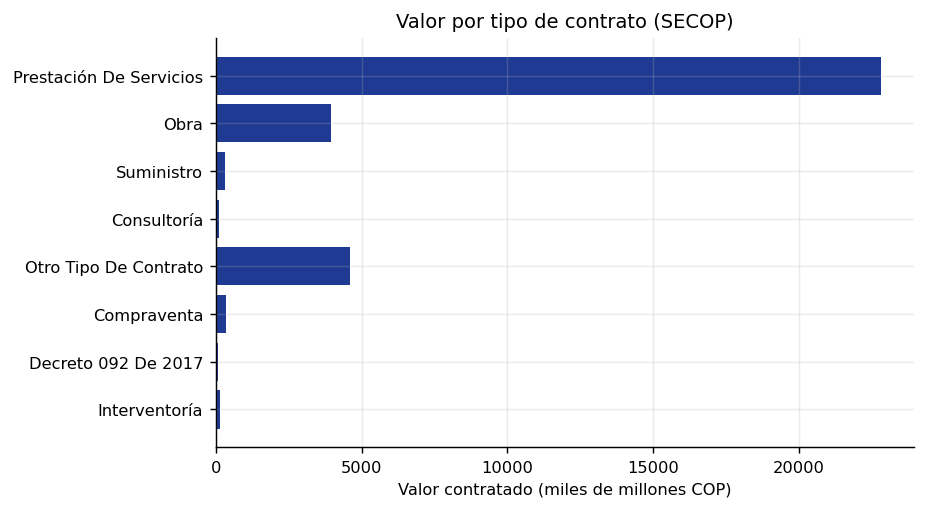
\includegraphics[width=0.74\linewidth]{figs_cruce/S1_secop_tipo.png}
\caption{Valor contratado por tipo de contrato. La obra y otros tipos de contrato, pese a ser minoritarios en número, concentran montos elevados.}\label{fig:secoptipo}\end{figure}

\subsection{Modalidad de contratación}
La modalidad de contratación (Tabla~\ref{tab:secop_modalidad}) confirma la lectura anterior desde el ángulo del procedimiento. La \textbf{contratación directa} y el \textbf{régimen especial} ---las vías habituales de los contratos de prestación de servicios--- son las que vinculan al grueso de los egresados, mientras que la \textbf{licitación pública}, reservada a los contratos de mayor cuantía, concentra una porción desproporcionada del valor (el 54,6\,\%) pese a su menor frecuencia. El egresado-contratista típico no compite en grandes licitaciones: es contratado de forma directa o por régimen especial para prestar un servicio profesional, y solo un puñado de vínculos pasa por la licitación que mueve las sumas mayores.

\begin{table}[H]\centering\footnotesize
\caption{Contratación de los graduados por \textbf{modalidad de contratación}.}\label{tab:secop_modalidad}
\begin{tabular}{lrrrr}
\toprule
\rowcolor{ustaazul}\textbf{\color{white}Modalidad} & \textbf{\color{white}Proveedores} & \textbf{\color{white}Contratos} & \textbf{\color{white}Valor} & \textbf{\color{white}\% valor} \\
\midrule
Licitación Pública & 239 & 790 & \$36.0 bill. & 54.6 \\
Contratación Régimen Especial & 3,431 & 14,279 & \$11.0 bill. & 16.7 \\
Contratación Directa & 26,211 & 166,002 & \$6.4 bill. & 9.7 \\
Régimen Especial & 7,279 & 29,195 & \$6.1 bill. & 9.3 \\
Contratación Directa (Ley 1150 De 2007) & 26,826 & 117,781 & \$4.4 bill. & 6.7 \\
Selección Abreviada De Menor Cuantía (Ley 1150 De 2007) & 528 & 2,373 & \$423.3 mil mill. & 0.6 \\
Contratación Régimen Especial (Con Ofertas) & 51 & 112 & \$247.0 mil mill. & 0.4 \\
Selección Abreviada De Menor Cuantía & 111 & 588 & \$228.9 mil mill. & 0.3 \\
\bottomrule
\end{tabular}
\end{table}

\subsection{Nivel de la entidad contratante}
Aquí emerge uno de los contrastes más instructivos del capítulo. Como muestran la Tabla~\ref{tab:secop_nivel} y la Figura~\ref{fig:secopnivel}, el \textbf{67,8\,\%} de los contratos de los graduados se firma con entidades del \textbf{orden territorial} (gobernaciones, alcaldías, entidades departamentales y municipales), pero esos contratos representan apenas el \textbf{38,1\,\%} del valor. A la inversa, las entidades del \textbf{orden nacional} suscriben solo el 32,2\,\% de los contratos pero acumulan el \textbf{61,9\,\%} del valor. Dicho de otro modo: el egresado trabaja, en su día a día, sobre todo para el Estado local ---que es quien le da dos de cada tres contratos---, mientras que las sumas verdaderamente grandes provienen de los vínculos con el nivel nacional.

\begin{table}[H]\centering\footnotesize
\caption{Contratación de los graduados por \textbf{nivel de la entidad} contratante.}\label{tab:secop_nivel}
\begin{tabular}{lrrrr}
\toprule
\rowcolor{ustaazul}\textbf{\color{white}Nivel de la entidad} & \textbf{\color{white}Contratos} & \textbf{\color{white}\% contratos} & \textbf{\color{white}Valor} & \textbf{\color{white}\% valor} \\
\midrule
Nacional & 111,804 & 32.2 & \$40.8 bill. & 61.9 \\
Territorial & 235,175 & 67.8 & \$25.1 bill. & 38.1 \\
(sin dato) & 118 & 0.0 & \$1.9 mil mill. & 0.0 \\
\bottomrule
\end{tabular}
\end{table}

\begin{figure}[H]\centering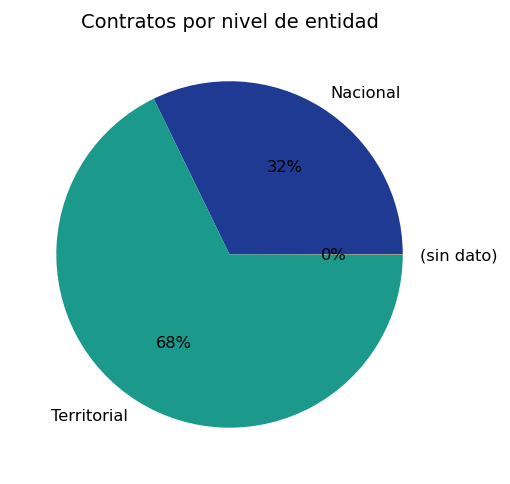
\includegraphics[width=0.50\linewidth]{figs_cruce/S3_secop_nivel.png}
\caption{Distribución de los contratos de los graduados según el nivel de la entidad contratante.}\label{fig:secopnivel}\end{figure}

\subsection{Concentración del valor en pocos contratos}
Antes de leer cualquier cifra de valor agregado conviene una cautela estadística. El valor total contratado ---del orden de \$65,9 billones--- está \textbf{fuertemente dominado por unos pocos atípicos}: el 10\,\% de proveedores de mayor monto concentra el \textbf{76,6\,\%} de todo el valor, y un \emph{único} documento aporta por sí solo \$22,2 billones, más de un tercio del total. Excluyéndolo, el agregado cae a \$43,7 billones. La mediana, en cambio, se sitúa en unos \textbf{\$113 millones} por proveedor, una cifra mucho más representativa del contratista real y dos órdenes de magnitud por debajo de los grandes montos que inflan la suma.

\begin{cajaobs}
Las sumas de valor deben leerse con prudencia. Un solo documento aporta más de un tercio del valor agregado, casi con certeza una colisión de identidad entre una cédula de graduado y una estructura de gran tamaño, o un contrato administrado a nombre de persona natural. Por ello, a lo largo del capítulo se privilegian las medidas robustas ---el número de proveedores, el número de contratos y la mediana de valor--- sobre las sumas, sensibles a estos atípicos. Un grupo reducido de megacontratos basta para desplazar el agregado en varios billones de pesos, de modo que cualquier comparación entre carreras o territorios que descanse en valores totales arrastra ese sesgo; la mediana, insensible a los extremos, ofrece el retrato fiel del egresado-contratista. La verificación de los megacontratos por documento queda como tarea de depuración pendiente.
\end{cajaobs}

\subsection{Contratación por carrera}
La Tabla~\ref{tab:secop_carrera} ordena los programas por número de graduados proveedores y revela una jerarquía nítida. El \textbf{Derecho} domina con holgura la contratación pública: \textbf{8.284} de sus egresados son proveedores del Estado y acumulan \textbf{74.243} contratos, una preeminencia coherente con la naturaleza jurídica de buena parte de la actividad estatal. Le siguen la Especialización en Derecho Administrativo (3.317 proveedores), la \textbf{Ingeniería Civil} (2.159) y la \textbf{Arquitectura} (1.882), volcadas a la obra y la consultoría públicas, y más atrás la \textbf{Odontología} (907), cuya presencia delata la contratación de servicios de salud por parte de entidades territoriales. Es revelador, además, que sean las \textbf{especializaciones} ---en particular la Especialización en Derecho Administrativo, con una mediana de \$173,9 millones--- las que exhiben las medianas de valor más altas: el posgrado no solo da acceso a la contratación, sino a contratos de mayor cuantía individual.

\begin{table}[H]\centering\footnotesize
\caption{Contratación pública por \textbf{carrera}: programas con más graduados proveedores.}\label{tab:secop_carrera}
\begin{tabular}{lrrrr}
\toprule
\rowcolor{ustaazul}\textbf{\color{white}Programa (carrera)} & \textbf{\color{white}Proveedores} & \textbf{\color{white}Contratos} & \textbf{\color{white}Valor (mediana)} & \textbf{\color{white}Valor total} \\
\midrule
Derecho & 8,284 & 74,243 & \$147.7 mill. & \$14.1 bill. \\
Especializacion En Derecho Admin & 3,317 & 33,795 & \$173.9 mill. & \$1.1 bill. \\
Ingenieria Civil & 2,159 & 14,884 & \$114.6 mill. & \$2.5 bill. \\
Arquitectura & 1,882 & 13,333 & \$77.5 mill. & \$4.8 bill. \\
Economia & 1,230 & 9,468 & \$136.3 mill. & \$22.7 bill. \\
Contaduria Publica & 1,227 & 8,868 & \$77.0 mill. & \$339.3 mil mill. \\
Psicologia & 1,221 & 8,811 & \$102.2 mill. & \$8.4 bill. \\
Especializacion En Auditoria De  & 1,090 & 10,734 & \$109.6 mill. & \$360.9 mil mill. \\
Negocios Internacionales & 1,068 & 6,303 & \$67.1 mill. & \$180.8 mil mill. \\
Cultura Fisica, Deporte Y Recrea & 1,008 & 6,852 & \$74.9 mill. & \$158.9 mil mill. \\
Odontologia & 907 & 5,410 & \$48.9 mill. & \$2.8 bill. \\
Ingenieria Ambiental & 761 & 5,203 & \$120.2 mill. & \$148.8 mil mill. \\
\bottomrule
\end{tabular}
\\[2pt]{\scriptsize\color{ustagris} Programa principal de cada proveedor. Ordenado por nº de proveedores. La mediana evita el sesgo de los megacontratos.}
\end{table}

\subsection{Objeto del contrato (UNSPSC)}
El tipo y la modalidad describen la \emph{forma} del contrato, pero no su \emph{objeto}. Para saber qué se contrata realmente hay que recurrir al clasificador internacional de bienes y servicios UNSPSC, que el SECOP Integrado no expone pero el SECOP~II sí. Cruzando a los graduados con el SECOP~II ---que cubre los contratos electrónicos, alrededor del 39\,\% del total--- se recupera el código UNSPSC de \textbf{136.800} de sus contratos. La Tabla~\ref{tab:secop_unspsc} muestra el resultado, y de entrada confirma una sospecha: la administración pública \emph{uniformiza}. El \textbf{79,3\,\%} de los contratos cae en una única categoría genérica de apoyo profesional y gestión ---encabezada por el código 80111600, ``servicios de personal''---, con la que el Estado rotula casi cualquier contrato de prestación de servicios, sea quien sea el contratista. El UNSPSC, al igual que el tipo de contrato, está dominado por ese cajón de sastre administrativo.

\begin{table}[H]\centering\footnotesize
\caption{Objeto contratado por los graduados según el clasificador \textbf{UNSPSC} (SECOP II).}\label{tab:secop_unspsc}
\begin{tabular}{lrr}
\toprule
\rowcolor{ustaazul}\textbf{\color{white}Categoría de objeto (UNSPSC)} & \textbf{\color{white}Contratos (SECOP II)} & \textbf{\color{white}\%} \\
\midrule
Apoyo profesional y gestión & 108.535 & 79,3\% \\
Cívico y político & 6.518 & 4,8\% \\
Jurídico & 6.143 & 4,5\% \\
Salud & 4.075 & 3,0\% \\
Ingeniería y TI & 3.679 & 2,7\% \\
Otros & 2.266 & 1,7\% \\
Educación & 2.174 & 1,6\% \\
Ambiental & 1.358 & 1,0\% \\
Financiero y contable & 1.016 & 0,7\% \\
\bottomrule
\end{tabular}
\\[2pt]{\scriptsize\color{ustagris} Solo contratos electrónicos (SECOP II), ~38\% del total. El código 80111600 (apoyo profesional) domina la categoría genérica.}
\end{table}

La señal disciplinar, sin embargo, no desaparece: se esconde en el residuo especializado. Si se aparta esa categoría genérica y se observa solo el objeto \emph{específico} de los contratos, emerge con nitidez la firma de cada profesión, como revela la Figura~\ref{fig:secopunspsc}. La Odontología y la Especialización en Auditoría de Salud contratan salud ---el 85,5\,\% del objeto especializado de esta última---, la Contaduría Pública se concentra en lo financiero y contable (62,1\,\%), la Ingeniería Civil y la Arquitectura en lo técnico y de ingeniería (65,0\,\% y 59,9\,\% respectivamente), y el Derecho ---junto con la Especialización en Derecho Administrativo--- en lo jurídico (61,7\,\%) y los asuntos cívicos y políticos. El objeto del contrato traduce, así, con fidelidad la disciplina de origen del egresado: cuando el Estado contrata especializadamente, contrata exactamente aquello para lo que cada profesión forma.

\begin{figure}[H]\centering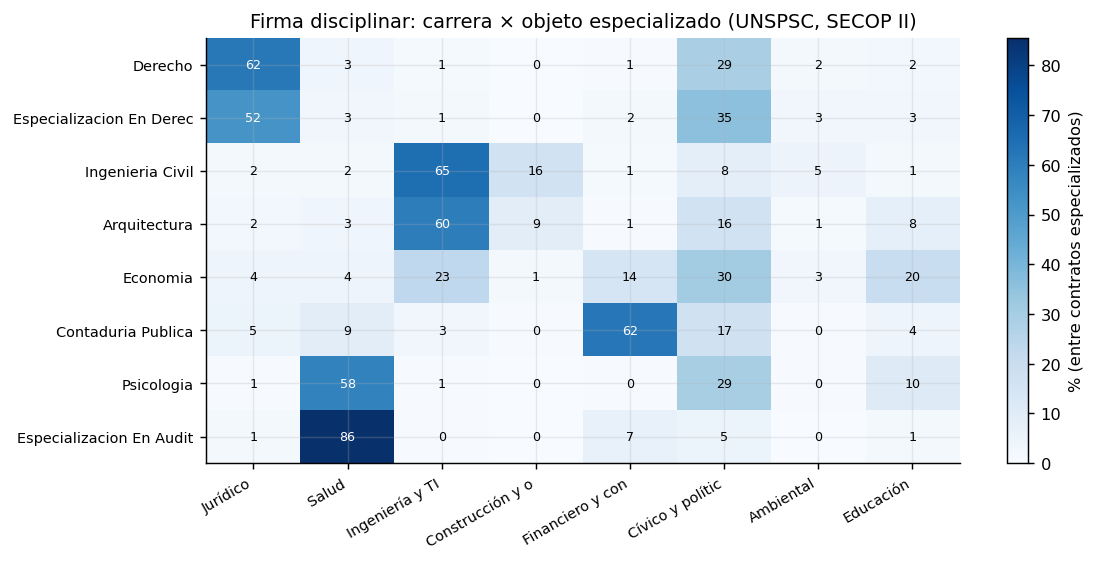
\includegraphics[width=0.94\linewidth]{figs_cruce/S6_secop_unspsc.png}
\caption{Objeto especializado de los contratos por carrera, según el código UNSPSC (\% sobre los contratos de cada carrera). Cada profesión deja su firma disciplinar una vez apartada la categoría genérica de apoyo profesional.}\label{fig:secopunspsc}\end{figure}

\subsection{Carrera y región de la contratación}
Superponer la carrera y el departamento de la entidad contratante (Figura~\ref{fig:secopcarrerareg}) combina las dos lecturas anteriores ---disciplinar y territorial--- en un solo mapa. El patrón general de arraigo regional se mantiene: cada profesión contrata sobre todo en los departamentos de sus sedes (Bogotá, Santander, Boyacá, Meta, Antioquia). Así, la Arquitectura concentra su contratación en Santander (36,8\,\%) y Boyacá (21,6\,\%), la Ingeniería Civil en Boyacá (31,3\,\%) y la Auditoría de Salud en Boyacá (33,5\,\%). Pero aparece un matiz disciplinar de interés: el \textbf{Derecho} muestra la mayor proyección nacional ---con el 42,6\,\% de sus contratos en Bogotá, sede de las entidades del orden nacional, y presencia repartida por Santander, Boyacá y el Meta---, mientras que profesiones más ligadas al territorio concentran su contratación en el departamento de su sede. La proyección nacional, así, no es homogénea: depende tanto de la disciplina como de la sede de origen.

\begin{figure}[H]\centering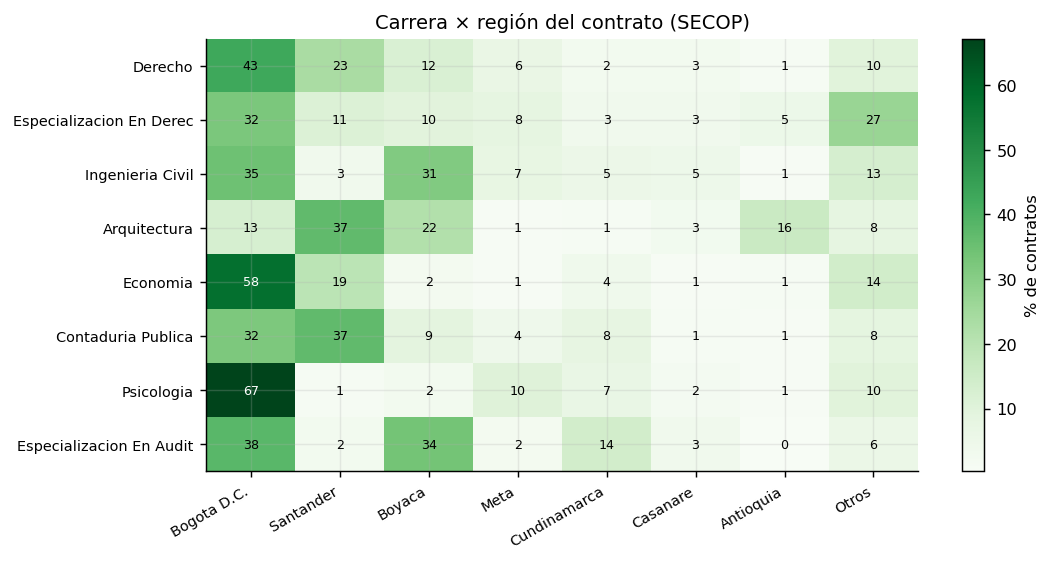
\includegraphics[width=0.92\linewidth]{figs_cruce/S5_secop_carrera_region.png}
\caption{Distribución regional de los contratos por carrera (\% de contratos por fila). El Derecho es la profesión de mayor alcance nacional.}\label{fig:secopcarrerareg}\end{figure}

\subsection{Síntesis del capítulo}
\begin{cajahallazgo}
El graduado tomasino se vincula con el Estado, ante todo, como prestador individual de servicios ---el 92,7\,\% de los contratos---, contratado de forma directa o por régimen especial y mayoritariamente por entidades territoriales, aunque el gran valor resida en unos pocos vínculos nacionales y en un puñado de megacontratos atípicos. La contratación nace en el Derecho y se extiende a las ingenierías, la arquitectura y la salud, con el posgrado como llave hacia contratos de mayor cuantía. El objeto contratado, una vez apartado el genérico administrativo, devuelve la firma disciplinar de cada profesión, y toda la huella aparece territorialmente arraigada: cada carrera contrata sobre todo en la región de su sede, siendo el Derecho la de mayor proyección nacional.
\end{cajahallazgo}

\noindent Queda, no obstante, una frontera por ampliar. El cruce con el SECOP~II que permitió recuperar el UNSPSC cubre solo los contratos electrónicos ---cerca del 39\,\% del total---, de modo que la lectura por objeto, aunque reveladora, descansa sobre una fracción de la contratación. Extender esa recuperación a la totalidad de los contratos, depurando además los megacontratos atípicos por documento, es la continuación natural de este capítulo.

\section{Matrícula mercantil (RUES)}

El segundo capítulo examina la huella mercantil del egresado. Al cruzar las cédulas de los cerca de 174.685 graduados de las seis sedes con el Registro Único Empresarial y Social, \num{37544} de ellos ---alrededor del 21,5\,\% del total--- aparecen como titulares de una matrícula mercantil. Como en el capítulo anterior, la pregunta deja de ser cuántos se registran en el RUES para volverse qué tipo de empresa crean, en qué sector, con qué supervivencia y desde qué carrera y territorio. Conviene advertir desde el principio una restricción que condiciona todo el capítulo: el enlace por cédula solo recupera a quien figura como persona natural comerciante, no a quien se registra en el RUES a través de una sociedad identificada por NIT, de modo que las cifras que siguen describen la matrícula mercantil individual y no la actividad societaria.

\subsection{Naturaleza jurídica de las empresas}
La Tabla~\ref{tab:rues_org} hace explícita esa restricción. La práctica totalidad de las matrículas enlazadas ---el 99,9\,\%--- corresponde a persona natural, sencillamente porque las sociedades se identifican con NIT y no con la cédula de sus socios, de modo que el cruce no las alcanza. La matrícula mercantil que este capítulo describe es, por tanto, la del egresado que registra negocio a su propio nombre ---el comerciante individual, el profesional independiente formalizado---, y no el de quien constituye una compañía. Se trata de un límite estructural más que de un hallazgo: el NIT queda fuera del alcance del enlace, así que la medición subestima la matrícula mercantil real. Cuanto sigue debe leerse con esa salvedad, que se retoma al cierre como límite principal.

\begin{table}[H]\centering\footnotesize
\caption{Matrículas de los graduados por \textbf{organización jurídica} (RUES).}\label{tab:rues_org}
\begin{tabular}{lr}
\toprule
\rowcolor{ustaazul}\textbf{\color{white}Organización jurídica} & \textbf{\color{white}\% de matrículas} \\
\midrule
Persona Natural & 99,9\% \\
Sociedad Limitada & 0,0\% \\
Otras Sociedades & 0,0\% \\
Empresas Asociativas De Trabajo & 0,0\% \\
Empresas Unipersonales & 0,0\% \\
\bottomrule
\end{tabular}
\\[2pt]{\scriptsize\color{ustagris} El cruce por cédula capta sobre todo persona natural; las sociedades con NIT no se enlazan por la cédula del socio.}
\end{table}

\subsection{Sector económico de las empresas}
Clasificando la actividad principal de cada matrícula por su código CIIU (Tabla~\ref{tab:rues_sector} y Figura~\ref{fig:ruessector}), el perfil sectorial del matriculado en el RUES tomasino es inequívoco. El comercio encabeza con holgura, con 9.535 matriculados en el RUES y el 25,4\,\% del total, seguido del alojamiento y la comida ---restaurantes, cafeterías, hospedaje--- con 3.841 matriculados en el RUES y el 10,2\,\%, y de las actividades profesionales y técnicas con 3.499 y el 9,3\,\%. Más atrás aparecen la industria manufacturera (5,0\,\%), la salud y la asistencia social (3,9\,\%), los servicios administrativos (3,3\,\%) y la construcción (2,9\,\%). El retrato es el de una matrícula mercantil de proximidad: comercio al por menor y servicios de consumo cotidiano, antes que actividades intensivas en capital o conocimiento.

\begin{table}[H]\centering\footnotesize
\caption{Sector económico de las empresas de los graduados, según \textbf{CIIU} (RUES).}\label{tab:rues_sector}
\begin{tabular}{lrr}
\toprule
\rowcolor{ustaazul}\textbf{\color{white}Sector económico (CIIU)} & \textbf{\color{white}Matriculados} & \textbf{\color{white}\%} \\
\midrule
Comercio & 9.535 & 25,4\% \\
Alojamiento y comida & 3.841 & 10,2\% \\
Profesionales y técnicas & 3.499 & 9,3\% \\
Industria manufacturera & 1.869 & 5,0\% \\
Salud y asistencia social & 1.454 & 3,9\% \\
Servicios administrativos & 1.251 & 3,3\% \\
Construcción & 1.077 & 2,9\% \\
Transporte y logística & 832 & 2,2\% \\
Educación & 796 & 2,1\% \\
Otros servicios & 789 & 2,1\% \\
\bottomrule
\end{tabular}
\\[2pt]{\scriptsize\color{ustagris} Sector de la actividad principal (división CIIU de la matrícula representativa de cada cédula).}
\end{table}

\begin{figure}[H]\centering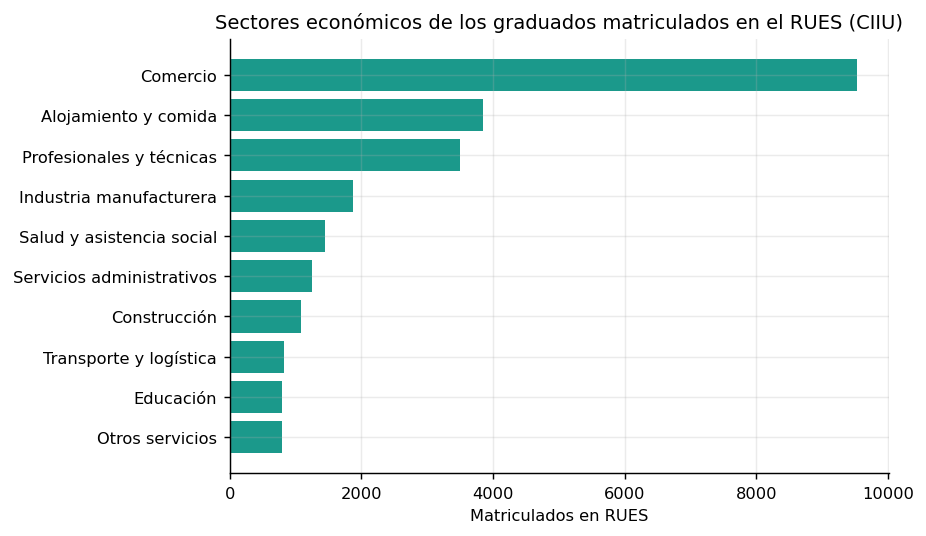
\includegraphics[width=0.74\linewidth]{figs_cruce/R1_rues_sector.png}
\caption{Sectores económicos (CIIU) de las empresas registradas por los graduados.}\label{fig:ruessector}\end{figure}

\subsection{Matrícula mercantil por carrera}
La Tabla~\ref{tab:rues_carrera} ordena los programas por número de graduados con matrícula mercantil. El Derecho vuelve a encabezar, con \num{3393} matriculados en el RUES, seguido de la Contaduría Pública (\num{2328}), la Economía (\num{1914}), los Negocios Internacionales (\num{1903}) y la Arquitectura (\num{1879}). La jerarquía reproduce en buena medida el tamaño de cada programa, pero la columna de empresa activa introduce un primer matiz: los Negocios Internacionales (44,7\,\%) y la Administración de Empresas (41,7\,\%) destacan muy por encima del promedio, mientras que programas como la Economía (24,7\,\%) o la Licenciatura en Educación Preescolar (16,3\,\%) se quedan por debajo. Como se verá, buena parte de ese contraste responde a la antigüedad de las matrículas y no a una solidez intrínseca del programa.

\begin{table}[H]\centering\footnotesize
\caption{Matrícula mercantil por \textbf{carrera}: programas con más graduados matriculados en el RUES.}\label{tab:rues_carrera}
\begin{tabular}{lrrr}
\toprule
\rowcolor{ustaazul}\textbf{\color{white}Programa (carrera)} & \textbf{\color{white}Matriculados} & \textbf{\color{white}Matrículas} & \textbf{\color{white}\% activa} \\
\midrule
Derecho & 3.393 & 3.951 & 29,0\% \\
Contaduria Publica & 2.328 & 2.809 & 27,0\% \\
Economia & 1.914 & 2.408 & 24,7\% \\
Negocios Internacionales & 1.903 & 2.275 & 44,7\% \\
Arquitectura & 1.879 & 2.392 & 30,8\% \\
Ingenieria Civil & 1.629 & 2.010 & 32,4\% \\
Especializacion En Derecho Adm & 1.248 & 1.493 & 21,4\% \\
Odontologia & 1.234 & 1.521 & 35,7\% \\
Administracion De Empresas & 1.180 & 1.372 & 41,7\% \\
Psicologia & 855 & 977 & 26,8\% \\
Administracion De Empresas Agr & 751 & 942 & 44,1\% \\
Licenciatura En Educacion Pree & 750 & 905 & 16,3\% \\
\bottomrule
\end{tabular}
\\[2pt]{\scriptsize\color{ustagris} Programa principal de cada graduado matriculado. Ordenado por nº de matriculados.}
\end{table}

\subsection{Sector económico por carrera}
Aquí surge el contraste más interesante con el capítulo de contratación pública. En el SECOP, cada profesión contrataba en su especialidad; en el RUES, la Figura~\ref{fig:ruescarrerasector} muestra que casi todas las carreras se registran en el RUES, ante todo, en el comercio: el egresado que crea empresa suele abrir un negocio, no ejercer su profesión por cuenta propia. El Derecho (42,4\,\% comercio), la Contaduría (48,7\,\%), la Economía (48,0\,\%) y los Negocios Internacionales (53,0\,\%) confirman ese patrón. Solo unas pocas disciplinas trasladan su formación al objeto de su empresa: la Odontología se registra en el RUES en salud (57,8\,\%), la Arquitectura en servicios profesionales y técnicos (36,0\,\%) y la Ingeniería Civil reparte su actividad entre el comercio (26,8\,\%) y la construcción (31,0\,\%). El título, que en la contratación pública determinaba el objeto del contrato, en la matrícula mercantil se diluye: salvo en la salud y en algunos servicios técnicos, el graduado se registra en el RUES como comerciante antes que como profesional de su disciplina.

\begin{figure}[H]\centering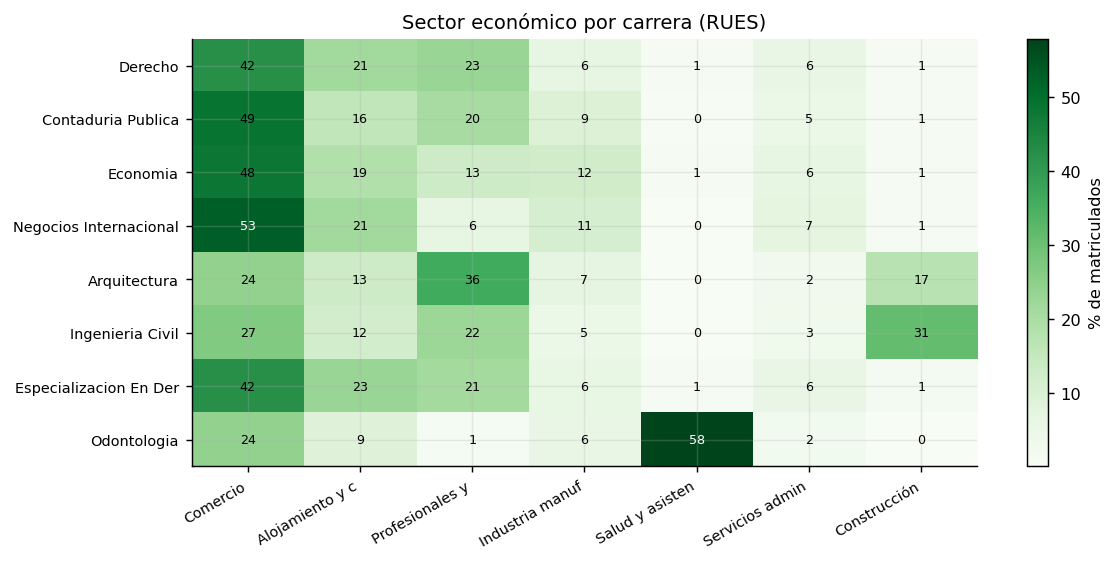
\includegraphics[width=0.94\linewidth]{figs_cruce/R2_rues_carrera_sector.png}
\caption{Sector económico de la empresa por carrera (\% de matriculados en el RUES por fila). El comercio domina en casi todos los programas; la salud y los servicios técnicos son las excepciones disciplinares.}\label{fig:ruescarrerasector}\end{figure}

\subsection{Supervivencia empresarial}
De las matrículas enlazadas, el 73,4\,\% figura como cancelada y solo el 24,7\,\% sigue activa (Tabla~\ref{tab:rues_estado}); contando por persona ---activa si conserva al menos una empresa viva---, \num{11125} matriculados en el RUES, el 29,6\,\%, mantienen actividad. Esa supervivencia no se reparte por igual entre carreras: como muestra la Figura~\ref{fig:ruessupcarrera}, programas como la Optometría (59,2\,\%), la Ingeniería Ambiental (56,0\,\%) o la Ingeniería Industrial (53,1\,\%) presentan las tasas de empresa activa más altas, frente a otros que apenas superan el 39\,\%.

\begin{table}[H]\centering\footnotesize
\caption{Estado de las matrículas de los graduados (RUES).}\label{tab:rues_estado}
\begin{tabular}{lr}
\toprule
\rowcolor{ustaazul}\textbf{\color{white}Estado de la matrícula} & \textbf{\color{white}\% de matrículas} \\
\midrule
Cancelada & 73,4\% \\
Activa & 24,7\% \\
Matrícula Cancelada Por Traslado De Domicilio & 0,8\% \\
Matrícula Cancelada Ley 1429 & 0,8\% \\
Matrícula Nueva, Constitución Por Traslado & 0,1\% \\
Matricula Inactiva Por Perdida De Calidad De Comerciante & 0,1\% \\
\bottomrule
\end{tabular}
\end{table}

\begin{figure}[H]\centering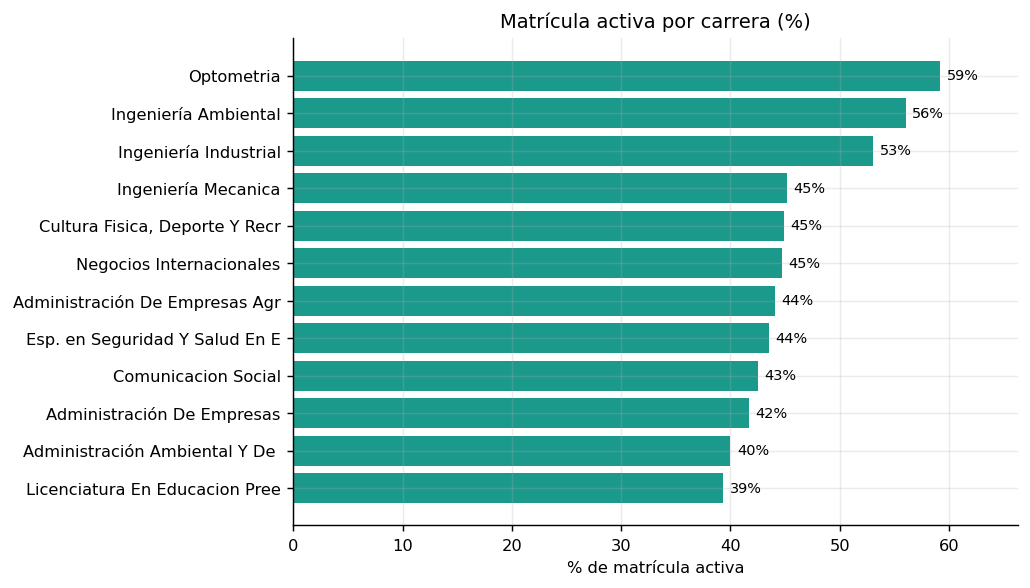
\includegraphics[width=0.74\linewidth]{figs_cruce/R3_rues_superv_carrera.png}
\caption{Porcentaje de graduados con empresa activa, por carrera (programas con un número suficiente de matriculados en el RUES).}\label{fig:ruessupcarrera}\end{figure}

Antes de sobreinterpretar esas diferencias conviene aislar un factor de confusión decisivo: la antigüedad. La Figura~\ref{fig:ruescohorte} relaciona la supervivencia con el quinquenio de la primera matrícula y el patrón es nítido: las empresas registradas hacia 2020 siguen activas en un 66,1\,\%, mientras que las de los años noventa apenas superan el 10\,\%. Es esperable ---una matrícula reciente ha tenido menos tiempo para cancelarse---, pero obliga a leer cualquier comparación de supervivencia controlando por la edad de la empresa: buena parte de las diferencias entre carreras y sedes refleja, en realidad, diferencias en la antigüedad de sus matrículas.

\begin{figure}[H]\centering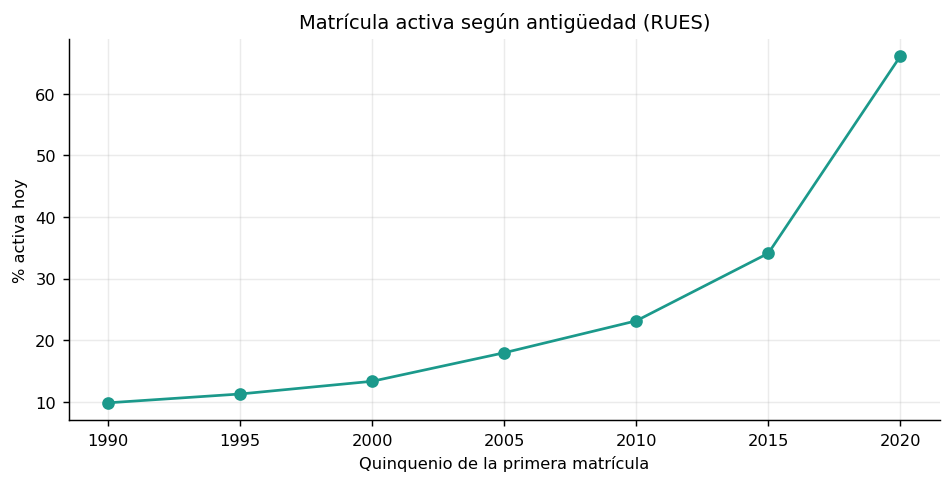
\includegraphics[width=0.74\linewidth]{figs_cruce/R4_rues_cohorte.png}
\caption{Porcentaje de empresas activas hoy según el quinquenio de la primera matrícula. La supervivencia observada depende fuertemente de la antigüedad.}\label{fig:ruescohorte}\end{figure}

\subsection{Supervivencia por sede}
Con esa cautela presente se leen las diferencias territoriales. En términos crudos, la tasa de empresa activa es del 24,1\,\% en Bogotá, del 31,6\,\% en Bucaramanga, del 40,1\,\% en Tunja, del 55,3\,\% en Villavicencio, del 33,5\,\% en Medellín y del 29,3\,\% en la VUAD. Tomado al pie de la letra, ese orden sugeriría una mayor solidez empresarial en Villavicencio; pero buena parte de la diferencia proviene de su juventud, pues, por ser una de las sedes más recientes, sus egresados registraron empresa más tarde y esas matrículas, más nuevas, han tenido menos tiempo para cancelarse.

Para separar la antigüedad del territorio conviene comparar sedes dentro de una misma cohorte de matrícula. La Figura~\ref{fig:ruessupseccoh} hace exactamente eso. Al controlar por el quinquenio de registro, la brecha se estrecha de manera notable ---en la cohorte 2015, por ejemplo, las tasas quedan en 35,7\,\% (Bucaramanga), 35,7\,\% (Tunja) y 42,9\,\% (Villavicencio), muy lejos de la diferencia cruda---, aunque Villavicencio conserva una ligera ventaja en todas las cohortes. La conclusión es matizada: la supervivencia territorial es, en su mayor parte, un artefacto de la antigüedad de las matrículas, sobre el que se monta una diferencia real pero modesta a favor de Villavicencio.

\begin{figure}[H]\centering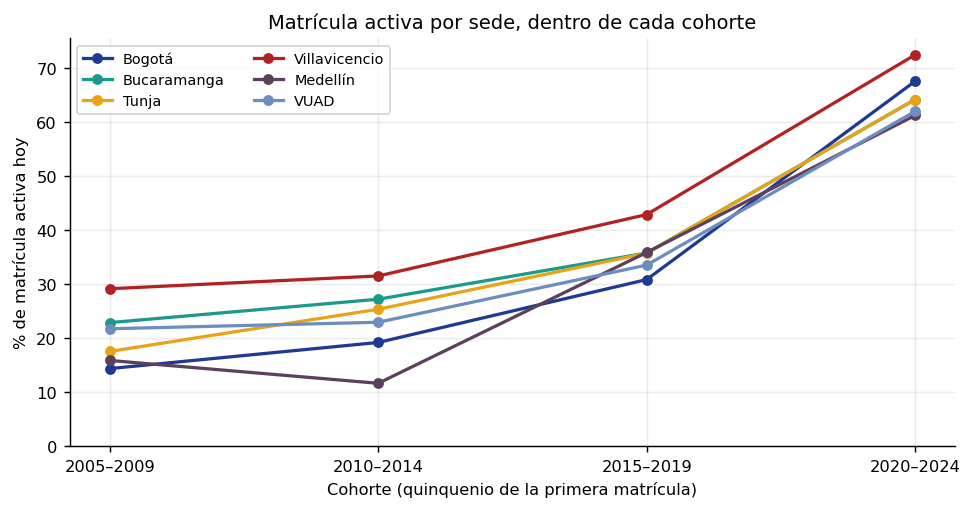
\includegraphics[width=0.78\linewidth]{figs_cruce/R5_rues_superv_seccional_cohorte.png}
\caption{Porcentaje de empresas activas por sede dentro de cada cohorte de primera matrícula. Al fijar la antigüedad, las diferencias territoriales se reducen sustancialmente.}\label{fig:ruessupseccoh}\end{figure}

\subsection{Síntesis del capítulo}
\begin{cajahallazgo}
La matrícula mercantil del egresado tomasino, tal como lo capta el RUES, es un fenómeno de persona natural volcado al comercio y los servicios de proximidad, con poco menos de un tercio de las empresas activas en la actualidad. A diferencia de la contratación pública, donde cada profesión contrata en su especialidad, en la matrícula mercantil la disciplina se diluye: salvo la salud y algunos servicios técnicos, el graduado abre negocio como comerciante antes que como profesional de su carrera. Y la supervivencia, más que un rasgo de cada programa o de cada sede, está gobernada por la antigüedad de la matrícula.
\end{cajahallazgo}

\noindent El límite de este capítulo es estructural y conviene reiterarlo. Al enlazar solo por cédula, el RUES capta la matrícula mercantil de persona natural pero deja fuera las sociedades constituidas con NIT, que son por lo común las de mayor escala y formalización. Las cifras de matrícula mercantil de este informe son, por tanto, un piso: la actividad societaria de los egresados ---probablemente la más relevante en términos económicos--- requiere un enlace adicional por nombre y representación legal que queda planteado como ampliación.

\section{Investigación (CvLAC)}

El tercer y último capítulo aborda la dimensión más selectiva de la huella del egresado: la actividad científica registrada en el Currículum de Vida Laboral y Académica (CvLAC) de Minciencias. Al cruzar los documentos de la base de \num{174685} graduados de las seis sedes con los perfiles CvLAC se validan \textbf{\num{2535} perfiles de investigador}, asociados a \textbf{\num{3403} registros} de coincidencia nombre--documento. Esos \num{2535} perfiles se corresponden con \textbf{\num{2547} graduados} de la base ---algunos perfiles enlazan con más de un registro documental---, y son estos \num{2547} egresados, el \textbf{1,5\,\%} del total, los que entran al cruce multidimensional del informe. Es, con diferencia, la dimensión de menor cobertura: frente a los miles de contratistas del SECOP o de matrículas del RUES, aquí hablamos de un par de millares de personas. No es una limitación del cruce sino el reflejo de una realidad, pues la investigación formal con hoja de vida en Minciencias es una actividad minoritaria entre cualquier población de profesionales. Por eso este capítulo no pregunta cuántos investigan, sino quiénes son: su nivel de formación, su reconocimiento por Minciencias, qué producen, en qué área del conocimiento y desde qué carrera y sede lo hacen.

\subsection{Validación de las coincidencias}
A diferencia del SECOP y del RUES, donde el enlace se hace por documento de forma exacta, el cruce con CvLAC exige una validación adicional, porque la coincidencia de un nombre o de una cédula no basta para afirmar que el investigador es, en efecto, un graduado tomasino. La validación se apoya en dos clases de evidencia que vinculan el perfil con la Universidad. La primera es la formación: el perfil CvLAC declara entre sus títulos un programa cursado en la Universidad Santo Tomás, lo que confirma el paso del investigador por la institución. La segunda es el grupo: el perfil pertenece a un grupo de investigación adscrito a la Universidad, lo que documenta un vínculo institucional vigente aunque el título no aparezca registrado. Un perfil se valida cuando reúne al menos una de estas dos evidencias. Conviene leer la cifra de \num{2535} validados como un \emph{piso} y no como un techo, pues quedan fuera de ella los investigadores cuyo paso por la Universidad no quedó consignado ni en sus títulos ni en su afiliación a un grupo, y que el procedimiento, deliberadamente conservador, prefiere no contar antes que contar de más.

\subsection{Nivel de formación}
La Tabla~\ref{tab:cvlac_nivel} ofrece el primer retrato del investigador validado, y es un retrato de alta cualificación. El \textbf{68,6\,\%} de los \num{2535} investigadores ha alcanzado un nivel de posgrado: la maestría es el nivel más frecuente, con el 40,4\,\% de los validados, seguida del doctorado, con el 18,5\,\%, y de la especialización, con el 9,8\,\%; a ellos se suma un pequeño núcleo de cuatro posdoctorados. El pregrado como nivel máximo queda en el 19,3\,\% y un 12,0\,\% no consigna su nivel. El contraste con las otras dos dimensiones es nítido: mientras el contratista del SECOP o el comerciante del RUES pueden ejercer con el solo título profesional, el investigador con hoja de vida en Minciencias es, de manera característica, un egresado que prolongó su formación más allá del pregrado. La investigación se concentra en la cúspide de la trayectoria académica.

\begin{table}[H]\centering\footnotesize
\caption{Nivel máximo de formación de los graduados validados en CvLAC.}\label{tab:cvlac_nivel}
\begin{tabular}{lrr}
\toprule
\rowcolor{ustaazul}\textbf{\color{white}Nivel máximo de formación} & \textbf{\color{white}Investigadores} & \textbf{\color{white}\%} \\
\midrule
Maestría & 1.023 & 40,4\% \\
Pregrado & 488 & 19,3\% \\
Doctorado & 469 & 18,5\% \\
No identificado & 303 & 12,0\% \\
Especialización & 248 & 9,8\% \\
Posdoctorado & 4 & 0,2\% \\
\bottomrule
\end{tabular}
\end{table}

\subsection{Categoría Minciencias}
El alto nivel de formación no se traduce, sin embargo, en un reconocimiento equivalente por parte de Minciencias. La Tabla~\ref{tab:cvlac_categoria} muestra que solo \textbf{\num{288} de los \num{2535} investigadores validados} (el 11,4\,\%) ostentan una categoría vigente en la convocatoria de medición; los \num{2247} restantes ---el 88,6\,\%--- figuran sin categoría. Entre los categorizados, la distribución dibuja la pirámide esperable: la base la forman los \textbf{164 investigadores Junior}, por encima se sitúan los \textbf{91 Asociados} y en la cima los \textbf{31 Senior}, a los que se añaden dos Eméritos. Que dos de cada tres validados tengan posgrado pero solo uno de cada diez alcance categoría revela una brecha entre la cualificación formal y el reconocimiento del sistema nacional de ciencia, que exige una producción sostenida y certificada que la mayoría de los egresados ---investigadores ocasionales o en etapas tempranas--- todavía no acumula.

\begin{table}[H]\centering\footnotesize
\caption{Categoría de investigador (Minciencias) de los graduados validados.}\label{tab:cvlac_categoria}
\begin{tabular}{lrr}
\toprule
\rowcolor{ustaazul}\textbf{\color{white}Categoría Minciencias} & \textbf{\color{white}Investigadores} & \textbf{\color{white}\%} \\
\midrule
Sin categoría & 2.247 & 88,6\% \\
Investigador Junior (IJ) & 164 & 6,5\% \\
Investigador Asociado (I) & 91 & 3,6\% \\
Investigador Senior (IS) & 31 & 1,2\% \\
Investigador Emérito (IE) & 2 & 0,1\% \\
\bottomrule
\end{tabular}
\end{table}

\begin{figure}[H]\centering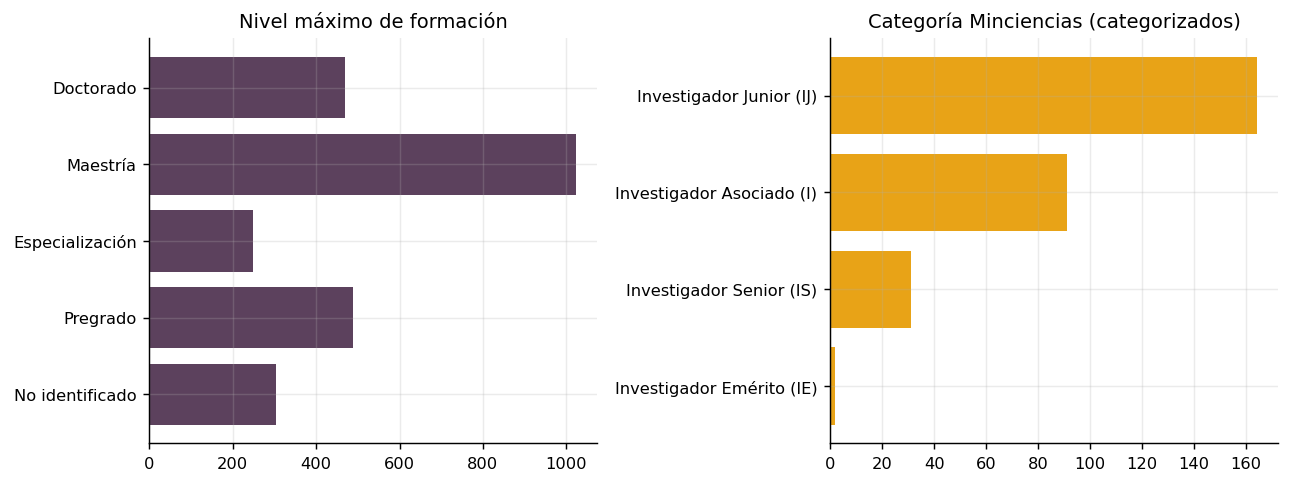
\includegraphics[width=0.90\linewidth]{figs_cruce/C1_cvlac_perfil.png}
\caption{Perfil del investigador validado: nivel máximo de formación y categoría Minciencias. El posgrado es mayoritario, pero la categorización es minoritaria.}\label{fig:cvlacperfil}\end{figure}

\subsection{Producción científica}
La Tabla~\ref{tab:cvlac_prod} agrega la producción declarada por los validados: \textbf{\num{13080} productos} registrados por los \num{2535} investigadores. La composición confirma una orientación marcadamente académica y, dentro de ella, la primacía indiscutida del \textbf{artículo}, que con \num{6434} productos concentra el 49,2\,\% de todo lo producido ---casi la mitad---. Le siguen los textos no científicos (18,5\,\%), los libros (10,1\,\%) y los capítulos de libro (6,9\,\%), de modo que la producción bibliográfica en sentido amplio domina por completo el panorama. Las formas de participación más aplicado ---consultorías, innovación de proceso, software--- aparecen en proporciones marginales, cada una por debajo del 2\,\%. El investigador tomasino produce, ante todo, conocimiento publicado en el formato canónico de la ciencia, y solo de manera residual transferencia tecnológica o productos de innovación.

\begin{table}[H]\centering\footnotesize
\caption{Producción científica de los graduados validados, por tipo de producto (CvLAC).}\label{tab:cvlac_prod}
\begin{tabular}{lrr}
\toprule
\rowcolor{ustaazul}\textbf{\color{white}Tipo de producto} & \textbf{\color{white}Productos} & \textbf{\color{white}\%} \\
\midrule
Artículos & 6.434 & 49,2\% \\
Textos no científicos & 2.422 & 18,5\% \\
Libros & 1.323 & 10,1\% \\
Capítulos de libro & 909 & 6,9\% \\
Demás trabajos & 497 & 3,8\% \\
Documentos de trabajo & 368 & 2,8\% \\
Otra prod. bibliográfica & 292 & 2,2\% \\
Consultorías & 264 & 2,0\% \\
Innovación de proceso & 164 & 1,3\% \\
Informes técnicos & 134 & 1,0\% \\
\bottomrule
\end{tabular}
\\[2pt]{\scriptsize\color{ustagris} Total de 13.080 productos registrados por los 2.535 investigadores validados.}
\end{table}

\begin{figure}[H]\centering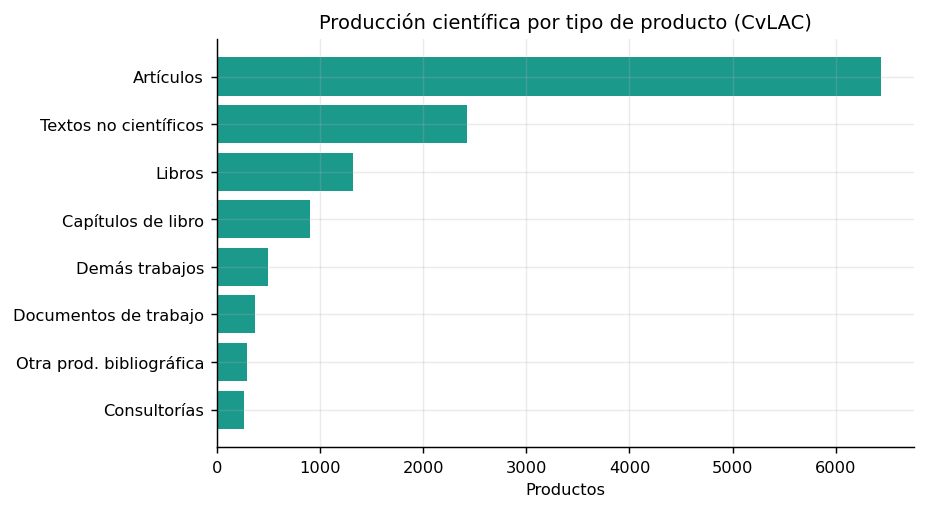
\includegraphics[width=0.74\linewidth]{figs_cruce/C2_cvlac_prod.png}
\caption{Producción científica de los graduados validados por tipo de producto. El artículo concentra cerca de la mitad de los \num{13080} productos.}\label{fig:cvlacprod}\end{figure}

\subsection{Categorización de las revistas}
La clasificación que declara CvLAC dice qué \emph{forma} tiene cada producto, pero no dónde se publica. Para caracterizar la calidad y el alcance de los artículos se extrajo el \textbf{ISSN} de cada uno ---\num{5640} menciones de revista en \num{1839} títulos distintos--- y se consultó cada revista en \textbf{OpenAlex}, el mayor catálogo bibliográfico abierto. El \textbf{82,5\,\%} de los artículos se publica en revistas indexadas en OpenAlex; de ellos, casi seis de cada diez (\textbf{59,5\,\%}) corresponden a revistas \textbf{colombianas} y un \textbf{55,1\,\%} a revistas de \textbf{acceso abierto} registradas en DOAJ (Tabla~\ref{tab:cvlac_revistas}). El perfil que emerge es el de una producción de visibilidad sobre todo nacional y de vocación abierta, con una presencia internacional minoritaria pero real ---tras Colombia aparecen Estados Unidos, España, Reino Unido y Brasil como países de edición---.

\begin{table}[H]\centering\footnotesize
\caption{Categorización de los artículos de los graduados según la revista (OpenAlex).}\label{tab:cvlac_revistas}
\begin{tabular}{lrr}
\toprule
\rowcolor{ustaazul}\textbf{\color{white}Indicador} & \textbf{\color{white}Artículos} & \textbf{\color{white}\%} \\
\midrule
Artículos con ISSN identificado & 5.640 &  \\
Revistas distintas (ISSN únicos) & 1.839 &  \\
En revista indexada en OpenAlex & 4.652 & 82,5\% \\
En revista de acceso abierto (DOAJ) & 2.561 & 55,1\% \\
En revista colombiana & 2.766 & 59,5\% \\
\bottomrule
\end{tabular}
\\[2pt]{\scriptsize\color{ustagris} ISSN extraído de cada artículo en CvLAC y consultado en OpenAlex.}
\end{table}

Clasificadas por el campo de conocimiento de la revista (Figura~\ref{fig:cvlaccampo}), las \textbf{Ciencias Sociales} concentran con holgura el grueso de los artículos, seguidas de la Economía y las Finanzas, las Ciencias de la Computación, las profesiones de la salud, las artes y humanidades, la medicina y la psicología. La distribución por campo de las revistas reproduce, desde la óptica editorial, el mapa disciplinar que ya mostraban las grandes áreas de actuación: la investigación de los graduados tomasinos es, ante todo, de ciencias sociales y humanas, con núcleos especializados en salud e ingeniería. Para una lectura de calidad en clave nacional, este mismo ISSN permitiría un cruce posterior con la categorización de \emph{Publindex} (A1, A2, B, C), que aquí queda planteado como extensión.

\begin{figure}[H]\centering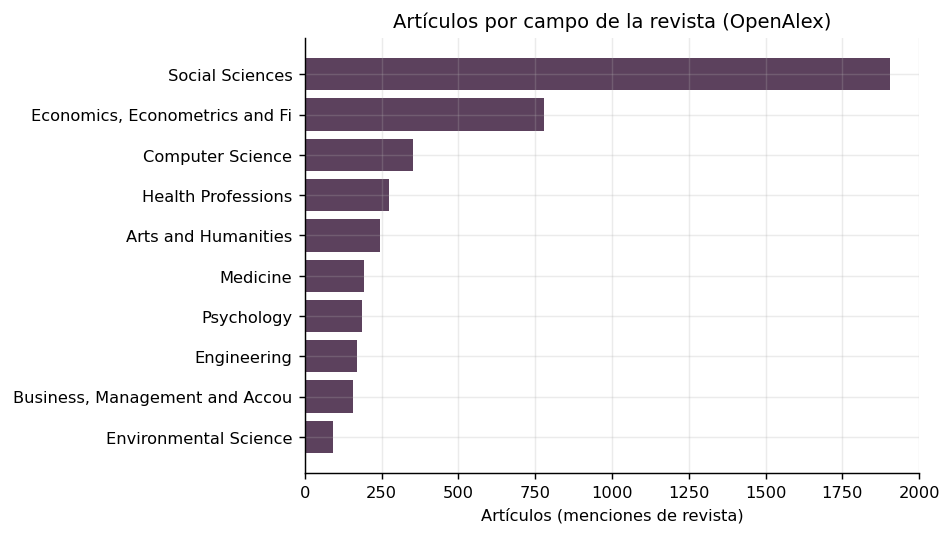
\includegraphics[width=0.74\linewidth]{figs_cruce/C4_cvlac_campo.png}
\caption{Artículos de los graduados validados según el campo de conocimiento de la revista (clasificación de OpenAlex).}\label{fig:cvlaccampo}\end{figure}

\subsection{Gran área de conocimiento}
Clasificando la producción de los investigadores por la gran área de conocimiento de Minciencias, el perfil global se inclina con claridad hacia las \textbf{Ciencias Sociales}, que reúnen \num{1345} investigadores ---más de la mitad del total---, seguidas a distancia por la \textbf{Ingeniería y Tecnología} (540) y las \textbf{Humanidades} (298); las Ciencias Médicas y de la Salud (166), las Ciencias Naturales (123) y las Ciencias Agrícolas (26) completan el cuadro. Más informativo que el agregado, sin embargo, es el cruce entre la carrera de origen y el área en que cada graduado investiga, que recoge la Figura~\ref{fig:cvlaccarreraarea}. Aquí se repite el patrón observado en el SECOP ---y que contrasta con la dispersión vista en el RUES---: cada carrera investiga en su área natural. El Derecho lo hace en Ciencias Sociales (el 93,6\,\% de sus investigadores), igual que la Economía (96,9\,\%) y la Psicología (92,1\,\%); las ingenierías se concentran en Ingeniería y Tecnología (el 99,1\,\% en Electrónica, el 86,7\,\% en Civil); la Cultura Física se vuelca a las Ciencias Médicas y de la Salud (76,9\,\%); y la Química Ambiental investiga, como cabe esperar, en Ciencias Naturales. La formación disciplinar de origen predice con notable fidelidad el territorio científico del egresado.

\begin{figure}[H]\centering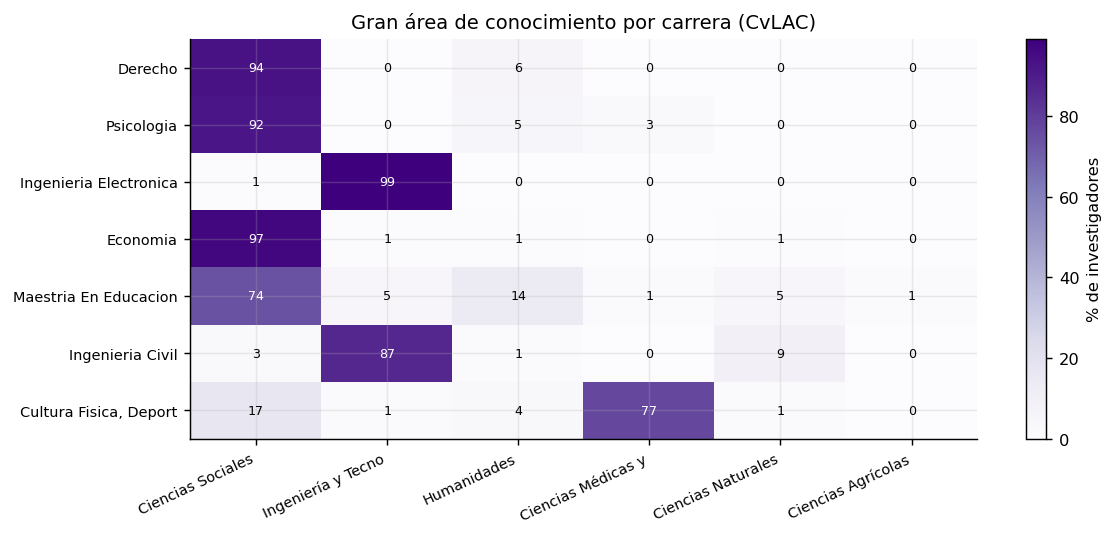
\includegraphics[width=0.92\linewidth]{figs_cruce/C3_cvlac_carrera_area.png}
\caption{Gran área de conocimiento de la investigación por carrera de origen (\% de investigadores por fila). Cada carrera investiga en su área natural.}\label{fig:cvlaccarreraarea}\end{figure}

\subsection{Investigación por carrera}
La Tabla~\ref{tab:cvlac_carrera} ordena los programas por número de graduados validados como investigadores y reproduce, en clave científica, jerarquías ya conocidas. El \textbf{Derecho} vuelve a encabezar, ahora con \textbf{273 investigadores}, una de las proporciones de doctorado más altas (24,1\,\%) y una mediana de dos productos por investigador. Le siguen la \textbf{Psicología} (115 investigadores), la \textbf{Ingeniería Electrónica} (113) y la \textbf{Economía} (99). Destaca la \textbf{Maestría en Educación}, que con 80 investigadores exhibe la mayor proporción de doctorado del cuadro (31,2\,\%) y la mediana de productos más alta (cuatro), un perfil coherente con un programa de posgrado orientado a la formación de investigadores. Más abajo aparecen las ingenierías Civil (78) y Ambiental (69), la Cultura Física (78), la Contaduría Pública (71), la Ingeniería de Telecomunicaciones (64), la Arquitectura (60) y los Negocios Internacionales (54). La investigación se reparte así entre las ciencias sociales, las ingenierías y, de forma destacada, los posgrados.

\begin{table}[H]\centering\footnotesize
\caption{Investigación por \textbf{carrera}: programas con más graduados validados en CvLAC.}\label{tab:cvlac_carrera}
\begin{tabular}{lrrr}
\toprule
\rowcolor{ustaazul}\textbf{\color{white}Programa (carrera)} & \textbf{\color{white}Investigadores} & \textbf{\color{white}\% doctorado} & \textbf{\color{white}Productos (mediana)} \\
\midrule
Derecho & 273 & 24,1\% & 2 \\
Psicologia & 115 & 13,0\% & 2 \\
Ingenieria Electronica & 113 & 8,0\% & 0 \\
Economia & 99 & 20,2\% & 1 \\
Maestria En Educacion & 80 & 31,2\% & 4 \\
Ingenieria Civil & 78 & 11,5\% & 0 \\
Cultura Fisica, Deporte Y Recr & 78 & 5,1\% & 0 \\
Contaduria Publica & 71 & 5,6\% & 0 \\
Ingenieria Ambiental & 69 & 1,4\% & 0 \\
Ingenieria De Telecomunicacion & 64 & 10,9\% & 0 \\
Arquitectura & 60 & 16,7\% & 2 \\
Negocios Internacionales & 54 & 0,0\% & 0 \\
\bottomrule
\end{tabular}
\\[2pt]{\scriptsize\color{ustagris} Programa de origen del graduado. Ordenado por nº de investigadores.}
\end{table}

\subsection{Investigación por sede}
La distribución de los investigadores validados por sede confirma la concentración esperable y la matiza con la densidad relativa. En números absolutos, \textbf{Bogotá} reúne \num{1434} investigadores ---más de la mitad---, seguida de Bucaramanga (528) y \textbf{Tunja} (388), y a distancia de Villavicencio (83), la VUAD (72) y Medellín (34). Bogotá y Tunja concentran, pues, el grueso de la actividad científica. Pero el número absoluto premia a las sedes de mayor tamaño y oculta la intensidad investigadora de las más pequeñas. Cuando los validados se ponen en relación con el volumen de graduados de cada sede, es \textbf{Tunja} la que muestra la mayor densidad relativa: produce proporcionalmente más investigadores que Bogotá pese a su menor tamaño. La sede de Boyacá emerge así no solo como la segunda en volumen, sino como la de vocación investigadora más intensa, un rasgo que el solo conteo absoluto dejaría invisible.

\subsection{Investigadores USTA fuera de la base de graduados}
El cruce con CvLAC arroja un hallazgo colateral que conviene registrar. Más allá de los \num{2535} perfiles validados como graduados, el ejercicio identifica \textbf{\num{3137} perfiles CvLAC adicionales con vínculo declarado a la Universidad Santo Tomás} ---por su formación, por su afiliación a un grupo de investigación o por ambas--- que no aparecen en la base de \num{174685} egresados. La explicación más probable es que se trate de docentes vinculados sin haberse graduado en la institución, de egresados de programas no incluidos en la base, o de graduados antiguos cuyo registro no quedó consignado en las fuentes disponibles. Sea cual sea su origen, este contingente de \num{3137} perfiles constituye un inventario valioso para futuros enlaces, pues señala la frontera entre la población medida en este informe y el universo más amplio de la comunidad investigadora tomasina.

\subsection{Síntesis del capítulo}
\begin{cajahallazgo}
La investigación es la dimensión más exigente y, a la vez, la mejor validada de la huella del egresado: solo \num{2535} graduados aparecen con hoja de vida en Minciencias, pero cada coincidencia se confirma por su formación o por su grupo en la Universidad. Es un colectivo de alta cualificación ---dos de cada tres tienen posgrado--- que, sin embargo, recibe poco reconocimiento formal del sistema nacional de ciencia, pues apenas uno de cada diez ostenta categoría Minciencias. Su producción se concentra en el formato canónico de la ciencia, con el artículo a la cabeza de los \num{13080} productos, y cada carrera investiga en su área natural: el Derecho y la Economía en ciencias sociales, las ingenierías en su campo técnico, la Química Ambiental en ciencias naturales. Bogotá y Tunja concentran la actividad, aunque Tunja despunta por su densidad investigadora. Y, como en las dimensiones anteriores, la cifra debe leerse como un piso y no como un techo, pues el procedimiento de validación, deliberadamente conservador, deja fuera a quien no dejó rastro de su paso por la Universidad.
\end{cajahallazgo}

\section{Participación multidimensional del egresado}

La participación de un egresado no se reduce a una sola huella. Una misma persona puede contratar con el Estado, registrar una empresa y figurar como investigadora reconocida, y hasta ahora cada una de esas huellas se observaba por separado, en fuentes distintas y sin un punto de cruce común. Esta sección reúne las tres dimensiones ---contratación pública (SECOP), actividad empresarial (RUES) y trayectoria investigativa (CvLAC)--- sobre una base de 174.685 graduados de las seis sedes de la Universidad Santo Tomás, consolidadas por cédula. El resultado es una lectura del egresado como un actor que deja, con frecuencia, más de una marca verificable en el país, y que permite preguntarse no solo cuántos dejan huella, sino con qué intensidad, desde qué nivel de formación, en qué sede y en qué combinación.

\subsection{Una tabla por persona}

El informe previo dejó pendiente justamente este paso, el de pasar de contar registros a contar personas. Un mismo graduado podía aparecer varias veces en SECOP, varias en RUES y de nuevo en CvLAC, de modo que sumar registros sobreestimaba el alcance real. Al consolidar las tres fuentes por cédula, cada graduado ocupa una sola fila y se le asocia el número de dimensiones en las que deja huella, de cero a tres. De los 174.685 graduados, 104.308 no registran huella en ninguna de las tres fuentes públicas consultadas, mientras que 70.377 aparecen al menos en una, como detalla la Tabla~\ref{tab:dist-dimensiones} y resume la Figura~\ref{fig:dimensiones}.

\begin{table}[H]
\centering
\caption{Distribución de graduados según el número de dimensiones de participación.}
\label{tab:dist-dimensiones}
\begin{tabularx}{0.78\linewidth}{Xrr}
\toprule
\rowcolor{ustaazul}\textbf{\color{white}Número de dimensiones} & \textbf{\color{white}Graduados} & \textbf{\color{white}Porcentaje} \\
\midrule
Ninguna (0) & 104.308 & 59,7\,\% \\
Una (1) & 58.001 & 33,2\,\% \\
Dos (2) & 12.149 & 7,0\,\% \\
Las tres (3) & 227 & 0,1\,\% \\
\midrule
\textbf{Total} & \textbf{174.685} & \textbf{100,0\,\%} \\
\bottomrule
\end{tabularx}
\end{table}

\begin{figure}[H]\centering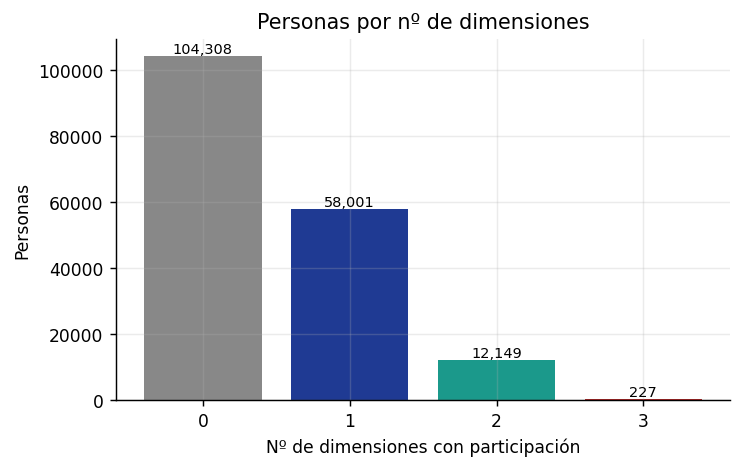
\includegraphics[width=0.78\linewidth]{figs_cruce/06_dimensiones.png}\caption{Distribución de graduados por número de dimensiones de participación.}\label{fig:dimensiones}\end{figure}

La lectura conviene hacerla con una cautela metodológica de fondo. Que seis de cada diez graduados no aparezcan en ninguna fuente no significa que carezcan de participación, sino que su trayectoria ---el empleo asalariado en el sector privado, el ejercicio liberal sin contratación estatal, la docencia, la migración al exterior--- transcurre por canales que estos tres registros públicos no capturan. Lo que el cruce mide no es, por tanto, la participación total del egresado, sino su huella en tres dominios concretos y verificables. Dentro de esos límites, la cifra es contundente.

\begin{cajahallazgo}
Cuatro de cada diez graduados (40,3\,\%) dejan huella verificable en al menos una de las tres dimensiones de participación, ya sea porque contratan con el Estado, porque se registran en el RUES o porque investigan. Es la primera vez que esta cifra se mide sobre la persona y no sobre el registro, lo que la convierte en una línea de base sólida para el seguimiento de los próximos años.
\end{cajahallazgo}

\subsection{Las combinaciones de participación}

Más allá del recuento por número de dimensiones, interesa saber qué facetas específicas se combinan en cada graduado, pues no es lo mismo contratar y registrarse en el RUES que investigar y contratar. La Tabla~\ref{tab:combinaciones} y la Figura~\ref{fig:combinaciones} descomponen los perfiles de quienes tienen al menos una huella.

\begin{table}[H]
\centering
\caption{Combinaciones de dimensiones entre los graduados con al menos una huella.}
\label{tab:combinaciones}
\begin{tabularx}{0.74\linewidth}{Xrr}
\toprule
\rowcolor{ustaazul}\textbf{\color{white}Combinación} & \textbf{\color{white}Graduados} & \textbf{\color{white}\%} \\
\midrule
Solo SECOP & 30.790 & 43,7\,\% \\
Solo RUES & 25.815 & 36,7\,\% \\
SECOP + RUES & 11.225 & 16,0\,\% \\
Solo CvLAC & 1.396 & 2,0\,\% \\
SECOP + CvLAC & 647 & 0,9\,\% \\
RUES + CvLAC & 277 & 0,4\,\% \\
SECOP + RUES + CvLAC & 227 & 0,3\,\% \\
\bottomrule
\end{tabularx}
\end{table}

\begin{figure}[H]\centering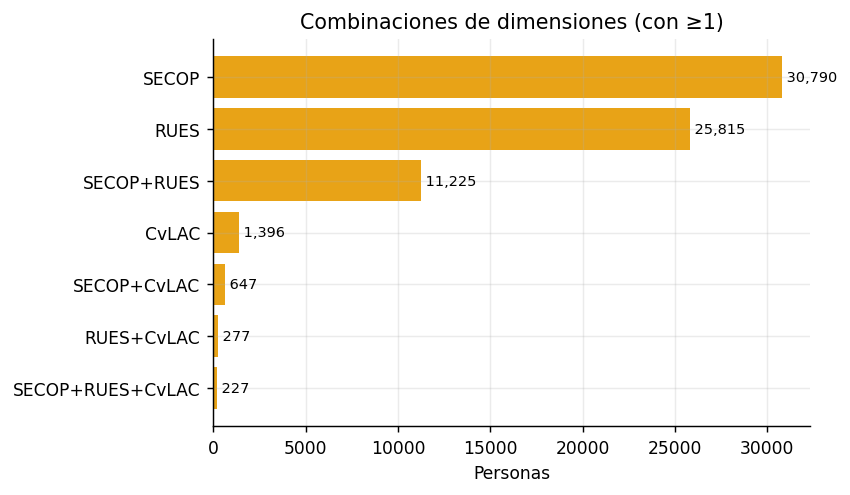
\includegraphics[width=0.78\linewidth]{figs_cruce/07_combinaciones.png}\caption{Combinaciones de participación entre los graduados que registran al menos una huella.}\label{fig:combinaciones}\end{figure}

Las huellas individuales dominan el panorama: la contratación pública en solitario reúne a 30.790 graduados (el 43,7\,\% de quienes dejan huella) y el registro empresarial en solitario a 25.815 (36,7\,\%). La combinación doble más frecuente es SECOP\,+\,RUES, con 11.225 graduados que a la vez contratan con el Estado y registran empresa, una cercanía natural porque muchos contratistas operan a través de compañías propias y comparten un mismo motor de actividad económica formal. Las combinaciones que incluyen investigación, en cambio, son marginales: 647 graduados suman SECOP y CvLAC, 277 reúnen RUES y CvLAC y solo 227 las tres dimensiones. La rareza de los perfiles con CvLAC confirma que la investigación reconocida es la más exigente y la menos extendida de las tres facetas.

\subsection{La intensidad de la huella}

Aparecer en una fuente y aparecer con fuerza son cosas distintas. Para matizar el recuento conviene mirar \emph{cuánta} huella deja quien deja huella, y el panorama es el de una amplia base de participación ligera coronada por una cola muy larga. La mediana del proveedor del Estado es de \textbf{5 contratos}, aunque el promedio sube a 8 por efecto de unos pocos contratistas con cientos de vínculos; la del matriculado en el RUES es de \textbf{una sola matrícula} mercantil; y la del investigador, de \textbf{2 productos} registrados, con un promedio de 5,7 que delata la presencia de unos cuantos investigadores muy prolíficos. En las tres dimensiones, por tanto, la norma es la huella modesta ---un puñado de contratos, una empresa, un par de publicaciones--- y la excepción son los perfiles intensivos que concentran la mayor parte del volumen. Esa asimetría, ya señalada en el capítulo de contratación a propósito de los megacontratos, recomienda leer la participación en términos de \emph{cuántas personas} participan antes que de los agregados, siempre dominados por los extremos.

\subsection{Participación y nivel de formación}

¿Pesa el posgrado en la huella del egresado? El cruce con la modalidad de formación ---disponible para los graduados de todas las sedes--- responde de forma afirmativa y nítida (Tabla~\ref{tab:modalidad-participación}). El graduado de posgrado deja huella en al menos una dimensión en el \textbf{43,9\,\%} de los casos, frente al \textbf{38,7\,\%} del graduado de pregrado, y la brecha se ensancha en la contratación pública, donde el posgrado alcanza el 30,5\,\% contra el 21,9\,\% del pregrado. También es más frecuente entre los posgraduados el perfil multidimensional, con un 8,8\,\% en dos o más dimensiones frente al 6,3\,\% del pregrado. La matrícula mercantil, en cambio, es prácticamente idéntica en ambos niveles, lo que sugiere que crear empresa depende menos del título y más de la iniciativa individual. La formación avanzada abre, sobre todo, las puertas de la contratación especializada con el Estado y de la investigación, las dos dimensiones donde la credencial posgradual rinde mayores frutos.

\begin{table}[H]
\centering
\caption{Tasas de participación según el nivel de formación (todas las sedes).}
\label{tab:modalidad-participación}
\begin{tabularx}{0.92\linewidth}{Xrrrrr}
\toprule
\rowcolor{ustaazul}\textbf{\color{white}Modalidad} & \textbf{\color{white}Graduados} & \textbf{\color{white}SECOP} & \textbf{\color{white}RUES} & \textbf{\color{white}CvLAC} & \textbf{\color{white}$\geq$1 dim.} \\
\midrule
Pregrado & 120.242 & 21,9\,\% & 21,9\,\% & 1,3\,\% & 38,7\,\% \\
Posgrado & 54.443 & 30,5\,\% & 20,6\,\% & 1,7\,\% & 43,9\,\% \\
\bottomrule
\end{tabularx}
\end{table}

\subsection{Participación por sede}

La participación tampoco se reparte por igual entre las sedes. La Tabla~\ref{tab:tasas-sede} compara las tasas por dimensión y dibuja perfiles diferenciados. Tunja encabeza la contratación pública, con el 45,2\,\% de sus graduados en SECOP, y también la investigación, con el 2,5\,\% en CvLAC, la tasa más alta del sistema; Villavicencio la sigue de cerca en contratación (38,0\,\%), lo que confirma el peso de las sedes regionales en el vínculo con el Estado. Bucaramanga lidera el registro empresarial (29,0\,\% en RUES). Bogotá, con más de cien mil graduados, presenta las tasas relativas más bajas en contratación y matrícula mercantil, un contraste que separa el volumen absoluto de la intensidad de la participación.

\begin{table}[H]
\centering
\caption{Tasas de participación por sede y dimensión.}
\label{tab:tasas-sede}
\begin{tabularx}{0.90\linewidth}{Xrrrr}
\toprule
\rowcolor{ustaazul}\textbf{\color{white}Sede} & \textbf{\color{white}Graduados} & \textbf{\color{white}SECOP} & \textbf{\color{white}RUES} & \textbf{\color{white}CvLAC} \\
\midrule
Bogotá & 104.468 & 20,0\,\% & 18,2\,\% & 1,5\,\% \\
Bucaramanga & 36.554 & 28,2\,\% & 29,0\,\% & 1,3\,\% \\
Tunja & 13.803 & 45,2\,\% & 24,8\,\% & 2,5\,\% \\
Villavicencio & 6.697 & 38,0\,\% & 24,2\,\% & 1,2\,\% \\
Medellín & 2.936 & 28,9\,\% & 17,8\,\% & 1,1\,\% \\
VUAD & 10.227 & 19,9\,\% & 23,3\,\% & 0,6\,\% \\
\bottomrule
\end{tabularx}
\\[2pt]{\scriptsize\color{ustagris} Aquí cada persona se asigna a una sola sede (su sede principal), de modo que los totales suman las 174.685 personas únicas. Difieren de la Tabla~\ref{tab:base_unificada}, que cuenta a quien tiene título en varias sedes dentro de cada una.}
\end{table}

\begin{figure}[H]\centering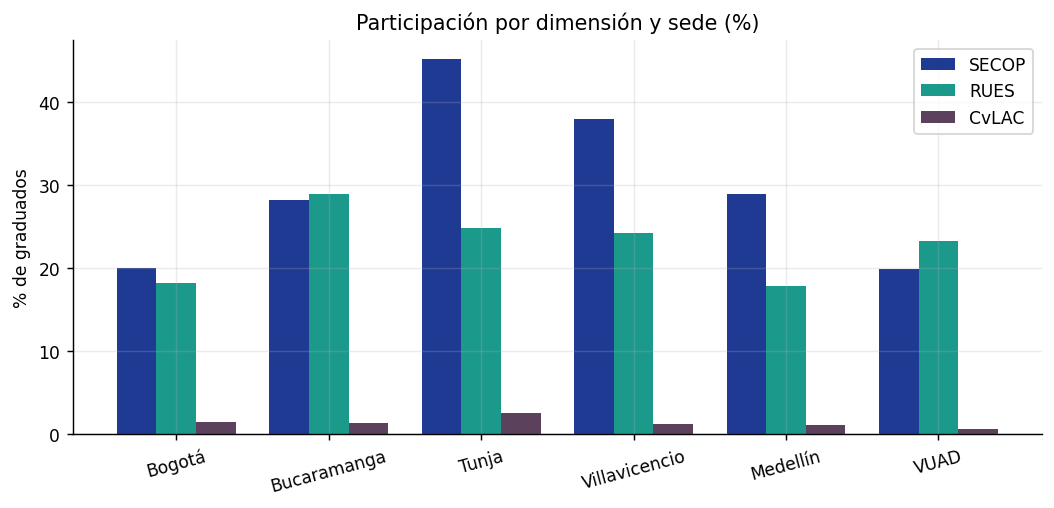
\includegraphics[width=0.80\linewidth]{figs_cruce/05_tasas_seccional.png}\caption{Tasa de graduados con huella por dimensión y sede.}\label{fig:tasas-seccional}\end{figure}

La composición por número de dimensiones (Figura~\ref{fig:dimensiones-seccional}) refuerza la lectura desde el ángulo de la acumulación. Tunja es la única sede donde los graduados con al menos una huella superan a quienes no tienen ninguna, y también la que concentra la mayor proporción de perfiles multidimensionales: el \textbf{14,2\,\%} de sus egresados deja huella en dos o más dimensiones, frente al 11,1\,\% de Villavicencio, el 9,2\,\% de Bucaramanga y apenas el 5,1\,\% de Bogotá. La geografía de la participación del egresado tomasino es, por tanto, desigual no solo en su frecuencia sino en su densidad, y conviene leerla siempre en proporciones antes que en conteos absolutos, dado el enorme peso numérico de la sede principal.

\begin{figure}[H]\centering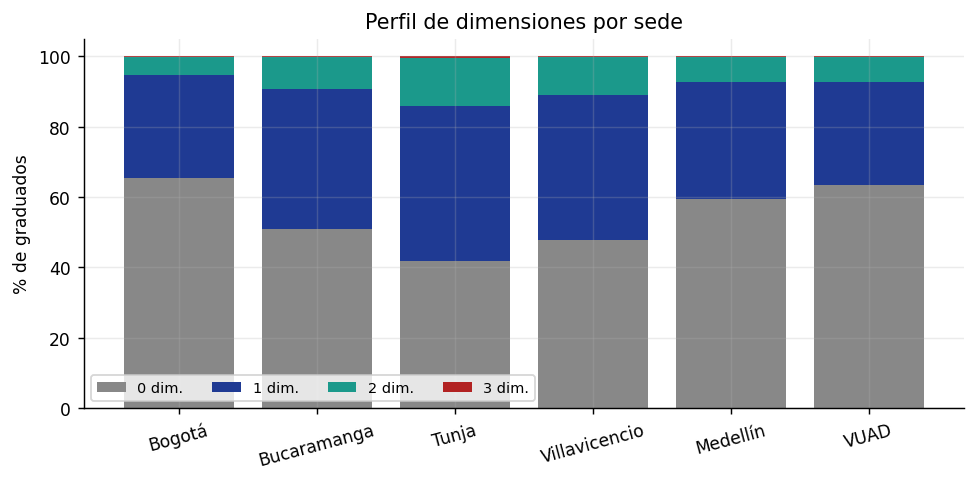
\includegraphics[width=0.80\linewidth]{figs_cruce/08_dimensiones_seccional.png}\caption{Perfil de graduados por número de dimensiones de participación (de cero a tres) en cada sede.}\label{fig:dimensiones-seccional}\end{figure}

\subsection{Participación según la cohorte de graduación}

La huella de un egresado se acumula con el tiempo, de modo que la participación por década de graduación debe leerse con cautela. La Tabla~\ref{tab:participación-decada} y la Figura~\ref{fig:participación-cohorte} muestran cómo la contratación pública crece de forma sostenida desde los años noventa hasta su máximo en la cohorte de 2010 (33,8\,\%), para descender al 28,6\,\% en la de 2020.

\begin{table}[H]
\centering
\caption{Tasas de participación según la década de graduación.}
\label{tab:participación-decada}
\begin{tabularx}{0.92\linewidth}{Xrrrr}
\toprule
\rowcolor{ustaazul}\textbf{\color{white}Década} & \textbf{\color{white}Graduados} & \textbf{\color{white}SECOP} & \textbf{\color{white}RUES} & \textbf{\color{white}CvLAC} \\
\midrule
1970 & 1.104 & 8,3\,\% & 27,4\,\% & 0,8\,\% \\
1980 & 9.355 & 11,1\,\% & 25,0\,\% & 0,8\,\% \\
1990 & 36.996 & 11,0\,\% & 22,4\,\% & 0,7\,\% \\
2000 & 35.939 & 24,9\,\% & 24,9\,\% & 1,6\,\% \\
2010 & 50.780 & 33,8\,\% & 21,9\,\% & 2,6\,\% \\
2020 & 40.490 & 28,6\,\% & 16,1\,\% & 0,8\,\% \\
\bottomrule
\end{tabularx}
\end{table}

\begin{figure}[H]\centering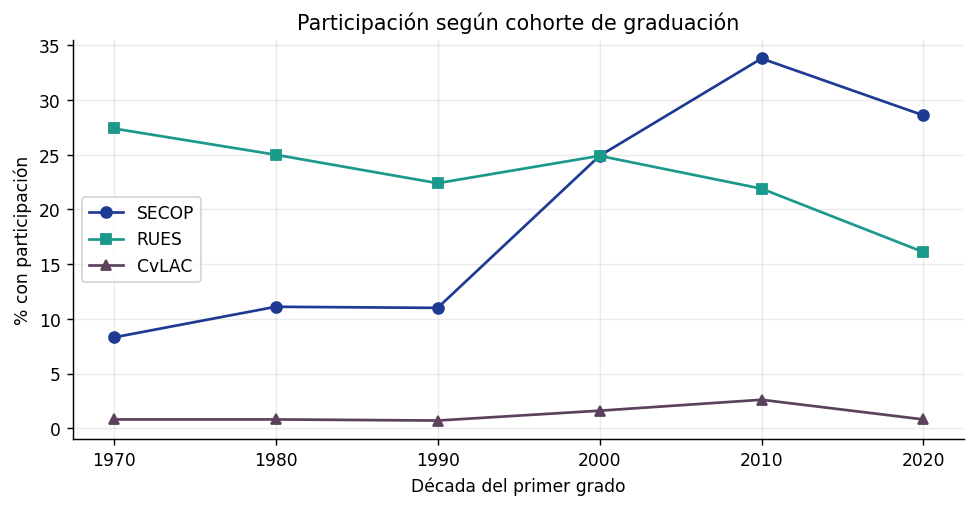
\includegraphics[width=0.80\linewidth]{figs_cruce/09_impacto_cohorte.png}\caption{Tasas de participación por dimensión según la década de graduación.}\label{fig:participación-cohorte}\end{figure}

La trayectoria investigativa sigue un patrón parecido al de la contratación, con su pico también en 2010 (2,6\,\%), mientras que el registro empresarial es más estable y cede algo en la cohorte más reciente. Dos factores explican esta forma. Por un lado, las cohortes recientes han tenido menos años para dejar huella, así que su menor tasa refleja exposición y no necesariamente potencial. Por otro, la cobertura del SECOP arranca a mediados de la década de 2000, lo que deprime artificialmente las tasas de contratación de las cohortes más antiguas, cuyos contratos previos no quedaron registrados en la plataforma. La caída de la cohorte de 2020 no debe interpretarse, por todo ello, como una pérdida de participación, sino como una maduración aún incompleta que solo los seguimientos de los próximos años podrán medir.

\subsection{El núcleo multidimensional}

El cruce por cédula permite, por fin, mirar de cerca a quienes concentran varias formas de participación a la vez. El solapamiento más frecuente es el de contratación y matrícula mercantil, con 11.452 graduados que figuran simultáneamente en SECOP y RUES. Pero la asociación más reveladora aparece alrededor de la investigación, la población más pequeña y exigente: entre los graduados con trayectoria en CvLAC, alrededor del \textbf{34,3\,\%} también contrata con el Estado y cerca del \textbf{19,8\,\%} también registra empresa, tasas muy por encima de las de la población egresada en general (Figura~\ref{fig:overlaps}). El investigador tomasino, lejos de ser una figura ensimismada, es con frecuencia un profesional activo que además contrata y se registra en el RUES.

\begin{figure}[H]\centering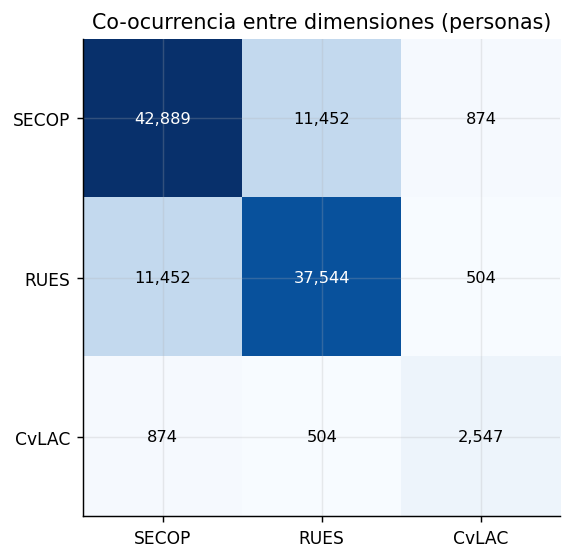
\includegraphics[width=0.62\linewidth]{figs_cruce/15_overlaps.png}\caption{Co-ocurrencia entre las tres dimensiones de participación (número de graduados).}\label{fig:overlaps}\end{figure}

En la cúspide de esa convergencia están los \textbf{227 graduados} que reúnen las tres dimensiones a la vez ---contratan, se registran en el RUES e investigan---, un núcleo diminuto pero significativo que ninguna fuente aislada habría podido identificar. Su distribución no es uniforme: 101 provienen de Bogotá, 60 de Bucaramanga y 49 de Tunja, y los 17 restantes de la VUAD (9), Villavicencio (6) y Medellín (2), de modo que Tunja aporta a este grupo de élite una proporción muy superior a su peso poblacional. Por programa, el Derecho domina con holgura (37 personas), seguido de la Especialización en Derecho Administrativo (14), la Arquitectura (11), la Maestría en Educación (10) y la Economía (9), una mezcla de profesiones liberales clásicas y de posgrados profesionalizantes. Conviene insistir en que toda esta convergencia es de \emph{asociación} y no de causalidad: los datos no permiten afirmar que investigar produzca mayor contratación o matrícula mercantil, sino que las tres facetas tienden a concentrarse en perfiles especialmente activos, formados y conectados.

\subsection{Participación por programa}

El tipo de huella depende, por último, en buena medida del programa cursado, como recoge el mapa de calor de la Figura~\ref{fig:heatmap-programa} y detalla la Tabla~\ref{tab:heatmap-programa}.

\begin{table}[H]
\centering
\caption{Tasas de participación por dimensión en programas seleccionados.}
\label{tab:heatmap-programa}
\begin{tabularx}{0.95\linewidth}{Xrrr}
\toprule
\rowcolor{ustaazul}\textbf{\color{white}Programa} & \textbf{\color{white}SECOP} & \textbf{\color{white}RUES} & \textbf{\color{white}CvLAC} \\
\midrule
Especialización en Derecho Administrativo & 57,7\,\% & 20,4\,\% & 0,8\,\% \\
Derecho & 44,1\,\% & 18,0\,\% & 1,5\,\% \\
Ingeniería Civil & 34,0\,\% & 25,4\,\% & 1,2\,\% \\
Cultura Física, Deporte y Recreación & 31,5\,\% & 17,9\,\% & 2,4\,\% \\
Arquitectura & 31,9\,\% & 32,0\,\% & 1,0\,\% \\
Psicología & 24,9\,\% & 17,2\,\% & 2,3\,\% \\
Odontología & 22,9\,\% & 31,1\,\% & 0,8\,\% \\
Economía & 17,5\,\% & 27,0\,\% & 1,5\,\% \\
Administración de Empresas & 14,3\,\% & 24,3\,\% & 0,4\,\% \\
Negocios Internacionales & 14,0\,\% & 24,8\,\% & 0,7\,\% \\
Contaduría Pública & 12,0\,\% & 22,8\,\% & 0,7\,\% \\
Lic. en Educación Preescolar y Promoción de la Familia & 3,0\,\% & 20,6\,\% & 0,1\,\% \\
\bottomrule
\end{tabularx}
\end{table}

\begin{figure}[H]\centering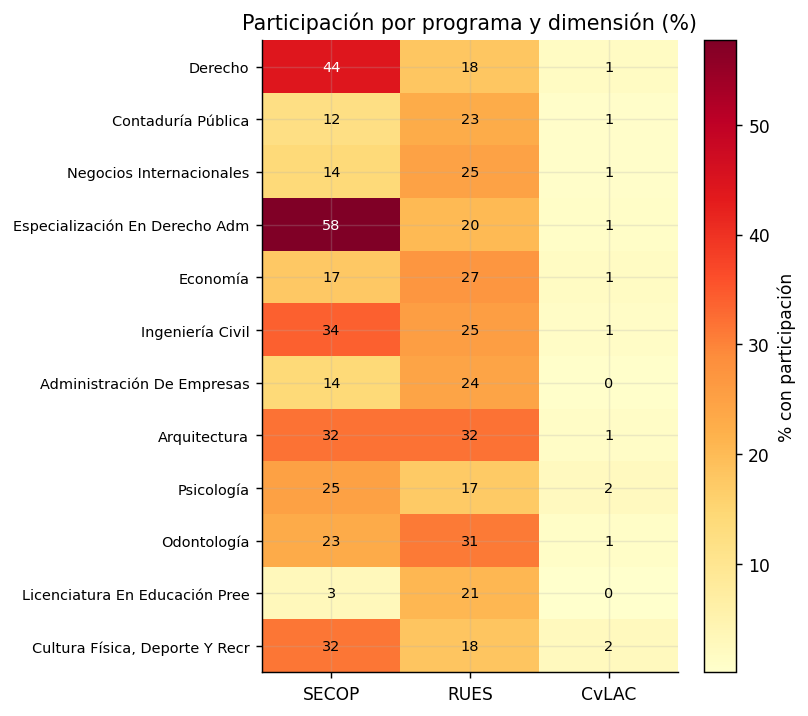
\includegraphics[width=0.66\linewidth]{figs_cruce/16_heatmap_programa.png}\caption{Mapa de calor de tasas de participación por programa y dimensión.}\label{fig:heatmap-programa}\end{figure}

Los programas jurídicos lideran la contratación pública: la Especialización en Derecho Administrativo alcanza el 57,7\,\% de sus graduados en SECOP y el Derecho el 44,1\,\%, seguidos de la Ingeniería Civil y la Arquitectura, disciplinas cuyo ejercicio gravita hacia el sector público. El registro empresarial se concentra en cambio en programas del área económica, del hábitat y de la salud, con Arquitectura (32,0\,\%), Odontología (31,1\,\%) y Economía (27,0\,\%) a la cabeza. La trayectoria investigativa, siempre minoritaria, es algo más visible en Cultura Física, Deporte y Recreación (2,4\,\%), Psicología (2,3\,\%) y Derecho (1,5\,\%). Programas de marcada vocación docente, como la Licenciatura en Educación Preescolar y Promoción de la Familia, muestran tasas bajas en las tres dimensiones, señal de que su participación se ejerce por canales ---la docencia, el aula--- que estas fuentes públicas no capturan. El cruce por programa convierte así el dato agregado en una herramienta de gestión curricular, al mostrar a cada facultad la vocación de participación predominante de sus egresados y, con ella, las dimensiones donde conviene reforzar el acompañamiento.

\begin{cajahallazgo}
El egresado tomasino deja huella sobre todo en una dimensión, pero existe un núcleo multidimensional que combina dos o las tres facetas: 12.149 graduados reúnen dos dimensiones y 227 las tres. Esa densidad crece con el posgrado y se concentra en Tunja, y la asociación entre contratación, matrícula mercantil e investigación reconocida ---en particular la presencia de los investigadores también en SECOP y RUES--- sugiere que estas formas de participación tienden a acompañarse antes que a excluirse. Se trata de una asociación y no de una relación causal, pero es justamente la convergencia que ninguna fuente aislada podía ver y que el Observatorio de Participación de Graduados pone por primera vez a la vista.
\end{cajahallazgo}

\section{Dimensión territorial de la participación}

Las tablas externas aportan una geografía que los registros académicos no contienen. El SECOP registra el departamento de la entidad que contrata a cada graduado y el RUES asocia cada empresa a una cámara de comercio. Al cruzar esa geografía con la sede de origen del egresado, la huella territorial de la Universidad deja de ser una abstracción y se vuelve medible: revela dónde trabaja y se registra en el RUES quien estudió en cada sede, hasta qué punto la participación de los 174.685 graduados se arraiga en los territorios donde la institución mantiene presencia, y cómo la modalidad a distancia proyecta esa huella mucho más allá de las ciudades sede.

\subsection{Dónde contratan los graduados (SECOP)}
La contratación pública de los graduados se concentra en los departamentos donde la Universidad tiene sede. Bogotá D.C. encabeza con 137.117 contratos, seguida de Santander con 56.876 y Boyacá con 41.709. El Meta aporta 19.694 y Cundinamarca 16.858, de modo que los territorios líderes corresponden a las regiones de las sedes de Bogotá, Bucaramanga, Tunja y Villavicencio, junto con el área de influencia inmediata de la capital. Por debajo aparecen Casanare con 9.447 contratos y Antioquia con 8.810, este último vinculado a la presencia en Medellín, seguidos de departamentos de menor peso como Norte de Santander, Cesar, Tolima, Valle del Cauca y Huila (Figura~\ref{fig:secopdep}). La actividad contractual de los egresados no se dispersa de forma homogénea por el país, sino que gravita alrededor de los nodos donde la institución forma profesionales.

\begin{figure}[H]\centering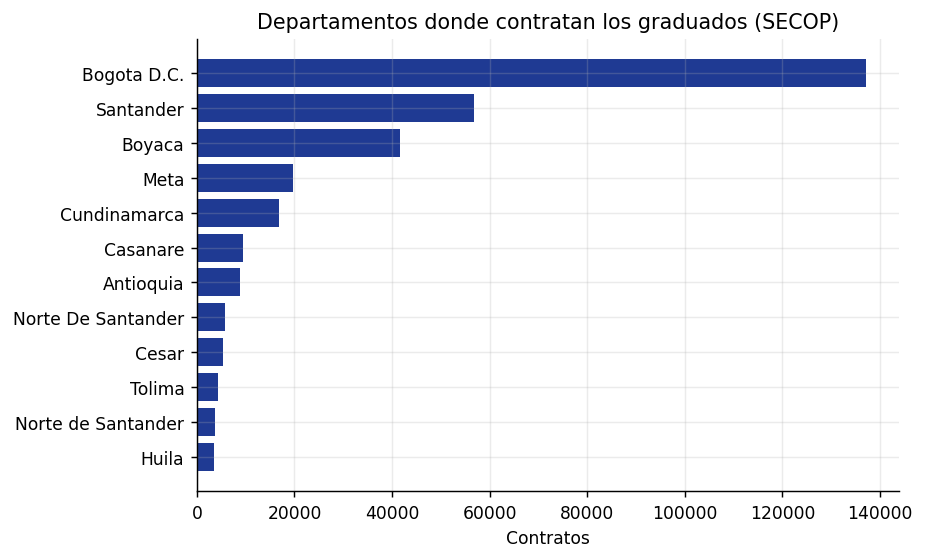
\includegraphics[width=0.78\linewidth]{figs_cruce/17_secop_departamento.png}
\caption{Departamentos de las entidades con las que contratan los graduados de la USTA (número de contratos, SECOP).}\label{fig:secopdep}\end{figure}

\subsection{Dónde registran empresa (RUES)}
La matrícula mercantil dibuja una geografía equivalente. La cámara de comercio de Bogotá registra 10.238 empresas de graduados, la de Bucaramanga 7.747, la de Tunja 3.326 y la de Villavicencio 2.516, todas correspondientes a ciudades sede de la Universidad. La cámara de Medellín para Antioquia suma 656 empresas, en línea con el tamaño de esa sede. Entre esas posiciones se intercalan cámaras del oriente y del piedemonte que prolongan el radio de influencia de las sedes ---Cúcuta con 1.151 empresas, Casanare con 821, Duitama con 815, Sogamoso con 642 y Barrancabermeja con 637, junto con Huila y Facatativá--- (Figura~\ref{fig:ruescam}). Tanto en la contratación pública como en la creación de empresas, los territorios de las sedes ocupan una y otra vez las primeras posiciones.

\begin{figure}[H]\centering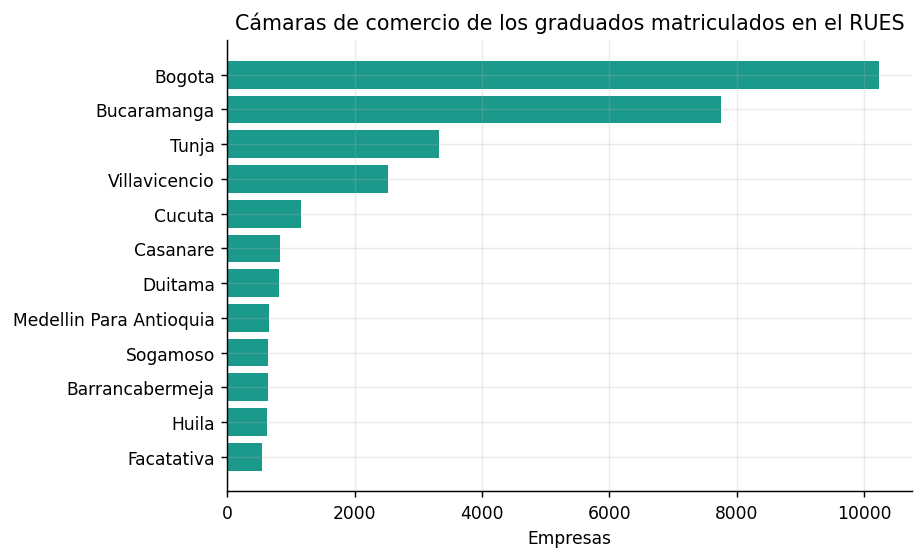
\includegraphics[width=0.78\linewidth]{figs_cruce/18_rues_camara.png}
\caption{Cámaras de comercio donde los graduados matriculados en el RUES registran sus empresas (RUES).}\label{fig:ruescam}\end{figure}

\subsection{Arraigo regional por sede}
Al descomponer la geografía por sede de origen, el arraigo se hace explícito: cada sede contrata y se registra en el RUES, sobre todo, dentro de su propio departamento. La Tabla~\ref{tab:arraigo} resume esa concentración y las Figuras~\ref{fig:secopreg} y~\ref{fig:ruesreg} la despliegan por completo. En la contratación pública, entre el 59\,\% y el 70\,\% de los contratos de cada sede se firma con entidades de su propio departamento; en la matrícula mercantil, la concentración es todavía mayor y culmina en Villavicencio, donde el 88,1\,\% de las empresas de sus graduados se registra en la cámara local, la cifra más alta de todo el sistema.

\begin{table}[H]
\centering
\caption{Concentración de la huella en el departamento de la sede de origen.}
\label{tab:arraigo}
\begin{tabularx}{0.93\linewidth}{Xlrr}
\toprule
\rowcolor{ustaazul}\textbf{\color{white}Sede} & \textbf{\color{white}Departamento} & \textbf{\color{white}Contratos en su depto.} & \textbf{\color{white}Empresas en su cámara} \\
\midrule
Bogotá & Bogotá D.C. & 61,8\,\% & 48,8\,\% \\
Bucaramanga & Santander & 59,6\,\% & 63,4\,\% \\
Tunja & Boyacá & 59,2\,\% & 60,7\,\% \\
Villavicencio & Meta & 66,7\,\% & 88,1\,\% \\
Medellín & Antioquia & 69,6\,\% & --- \\
\bottomrule
\end{tabularx}
\end{table}

\begin{figure}[H]\centering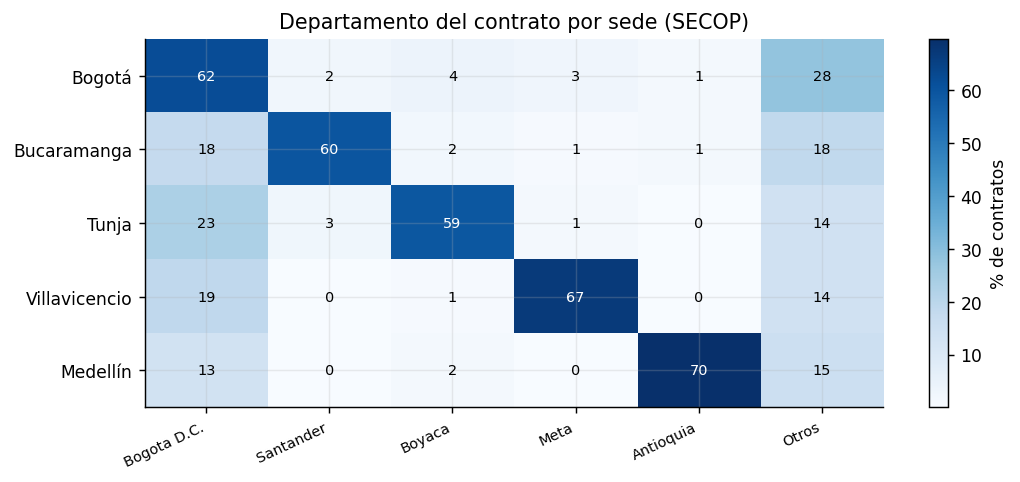
\includegraphics[width=0.85\linewidth]{figs_cruce/19_secop_seccional_region.png}
\caption{Distribución del departamento de contratación según la sede de origen del graduado (\% de contratos por fila, SECOP).}\label{fig:secopreg}\end{figure}

\begin{figure}[H]\centering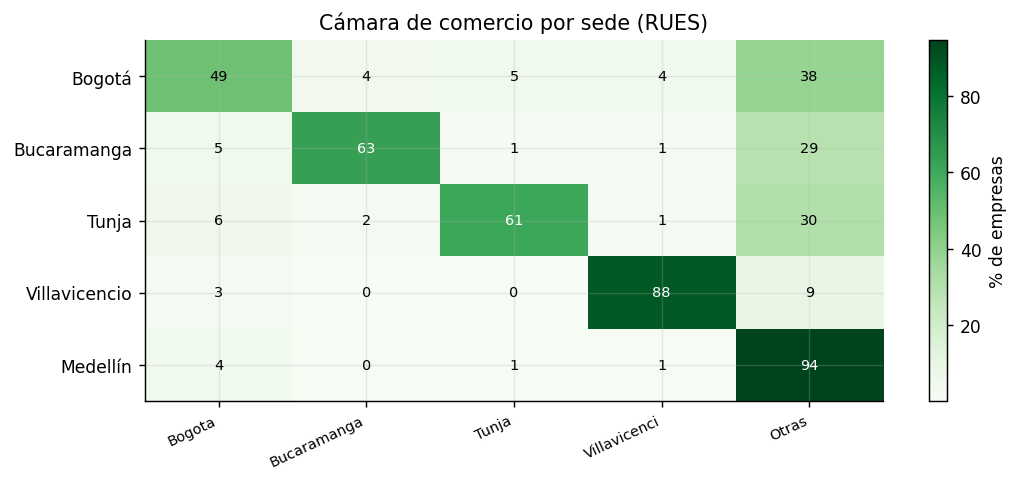
\includegraphics[width=0.85\linewidth]{figs_cruce/20_rues_seccional_camara.png}
\caption{Distribución de la cámara de comercio de registro según la sede de origen del graduado (\% de empresas por fila, RUES).}\label{fig:ruesreg}\end{figure}

Por encima de ese predominio regional, la capital opera como un segundo polo de atracción para todas las sedes. Tras su propio departamento, los graduados de Tunja dirigen el 23,1\,\% de sus contratos a entidades de Bogotá D.C., los de Bucaramanga el 17,7\,\%, los de Villavicencio el 18,7\,\% y los de Medellín el 13,4\,\%. Esa atracción no desplaza el arraigo local, pero refleja la gravitación natural de las entidades del orden nacional, concentradas en la capital, sobre los contratistas de todo el país. El mapa que resulta es de doble nivel: una base sólida de participación regional sobre la que se monta un vínculo secundario y común con el centro administrativo de la Nación.

\subsection{La huella nacional de la educación a distancia}
El patrón de arraigo regional encuentra su excepción ---y su complemento--- en la modalidad a distancia. Los graduados de los centros VUAD, que la Universidad sostiene en decenas de municipios sin campus presencial, no se concentran en un único departamento, sino que riegan su huella por todo el país. Sus contratos se reparten entre Bogotá D.C. (2.916), Boyacá (1.489), Casanare (1.179), Santander (1.065) y, de manera reveladora, departamentos donde la institución no tiene sede física, como Nariño (967), Quindío (956), el Meta (869) y Cundinamarca (710). Mientras las sedes presenciales irradian participación sobre su entorno inmediato, la educación a distancia proyecta la presencia de la Universidad sobre la geografía nacional, alcanzando regiones que de otro modo quedarían fuera de su radio. La huella territorial del egresado tomasino tiene, así, dos formas complementarias: la concentrada de las sedes presenciales y la difusa de la modalidad a distancia.

\begin{cajahallazgo}
La participación del egresado es profundamente regional. Lejos de dispersarse por todo el país, la contratación pública y la matrícula mercantil de los graduados se concentran en el departamento de su sede de origen, en proporciones que van del 59\,\% al 70\,\% en el SECOP y hasta el 88\,\% en el RUES, con Bogotá como único destino nacional compartido. Cada sede nutre de forma directa el tejido productivo e institucional de su territorio, de modo que la presencia de la Universidad en seis sedes se traduce en otros tantos polos de desarrollo regional, mientras la modalidad a distancia extiende esa huella a departamentos sin campus propio. La institución no solo forma profesionales, sino que actúa como motor del desarrollo de las regiones donde se asienta, retornando a cada territorio el talento que en él se ha formado.
\end{cajahallazgo}

\section{Discusión}

El valor de este trabajo no reside en describir SECOP, RUES y CvLAC en paralelo, sino en cruzarlas sobre una misma población de 174.685 graduados de las seis sedes. Tres tablas yuxtapuestas describen tres mundos; una sola tabla resuelta sobre la identidad de la persona describe una trayectoria. Esa diferencia, más conceptual que técnica, es la que separa un inventario de fuentes de un observatorio de participación. Sobre esa base, el cruce muestra que el 40,3\% de los graduados deja al menos un rastro en alguna de las tres dimensiones.

Donde existe una llave de identidad estable, el cruce es directo y masivo. El número de documento permite enlazar al graduado con su huella de contratación pública en SECOP y con su actividad como persona natural comerciante en RUES sin ambigüedad apreciable: por esa vía se confirman 42.889 graduados contratistas (24,6\%) y 37.544 matriculados en el RUES (21,5\%). La llave hace el trabajo y el cruce escala a decenas de miles de coincidencias verificables. El problema aparece donde la llave no existe: la plataforma CvLAC no expone el documento, de modo que el enlace solo puede intentarse por nombre, y coincidir por nombre es frágil por homónimos, variantes de tildes y nombres compuestos.

La salida no fue renunciar a la dimensión científica, sino sustituir la coincidencia por evidencia. En lugar de aceptar el emparejamiento por nombre como prueba suficiente, se exigió respaldo verificable adicional, formación declarada compatible con un programa de la USTA o vínculo con un grupo de investigación, antes de validar a una persona; el resultado son 2.547 investigadores confirmados. De ahí la enseñanza metodológica que atraviesa el ejercicio: la resolución de identidades es lo que convierte un inventario en un observatorio, porque sin una política explícita sobre cuándo dos registros son la misma persona el cruce es una ilusión de precisión. Esa misma operación es la que produce los 227 graduados presentes en las tres dimensiones a la vez.

El cruce reveló además una asociación que conviene subrayar con cautela. Entre los graduados validados en CvLAC, cerca del 34,3\% aparece también en SECOP y el 19,8\% en RUES: investigar, contratar y registrarse en el RUES no son trayectorias mutuamente excluyentes, sino que tienden a concurrir en las mismas personas. Se trata de una asociación, no de una relación causal, pues este artículo ejecutó el cruce pero no modeló el mecanismo; no puede afirmarse que investigar cause mayor contratación o matrícula mercantil, solo que ambos rasgos se observan juntos con una frecuencia que invita a estudiarlos. Por último, en CvLAC se adoptó un criterio deliberadamente conservador, que prefiere el falso negativo al falso positivo, de modo que las 2.547 personas confirmadas deben leerse como un piso y no como una estimación central de la participación investigativa real.

\section{Limitaciones y trabajo futuro}

\begin{itemize}\setlength\itemsep{2pt}
  \item El RUES solo capta a quien figura como persona natural comerciante, así que el graduado que se registra en el RUES a través de una sociedad identificada por NIT no se enlaza por su cédula y la dimensión empresarial queda subestimada, sobre todo en su tramo de mayor escala.
  \item La clasificación de bienes y servicios por código UNSPSC solo está disponible a partir de SECOP II, que cubre alrededor del 39\% de los contratos, por lo que el análisis sectorial de la contratación es todavía parcial.
  \item Al no disponer de documento, la identidad en CvLAC se valida combinando nombre y evidencia, sin confirmación caso a caso; conviene auditar manualmente una muestra contra la hoja de vida pública de cada persona para estimar la tasa de error del criterio.
  \item Falta incorporar el SNIES para enriquecer la caracterización académica y la cohorte de graduación para normalizar por antigüedad, de modo que se compare de forma justa a quien lleva décadas en el mercado con quien egresó hace pocos años, sin confundir madurez de trayectoria con mayor participación.
  \item Queda dar el salto del cruce al modelo, pues este artículo cruzó las fuentes pero analizarlas estadísticamente, con modelos de los determinantes de la participación y de supervivencia condicionada que estimen el tiempo hasta el primer contrato o el primer registro empresarial, exige más que conteos.
  \item Resta consolidar las tres dimensiones en un tablero unificado y automatizar la ingesta de las fuentes con una fecha de corte explícita, para que cada actualización sea reproducible y comparable con la anterior sin rehacer el proceso a mano.
\end{itemize}

\section{Nota de observaciones}

En coherencia con el registro evaluativo que ha caracterizado a este equipo, esta nota separa lo que el ejercicio efectivamente logró de lo que apenas deja planteado. El balance es deliberadamente prudente: se ejecutó el cruce de las tres fuentes sobre la población completa, y ese es un avance real; pero la ejecución del cruce no debe confundirse con su explotación analítica, que apenas comienza.

\begin{cajaobs}
\textbf{Alcance de los hallazgos}

El cruce de identidades se ejecutó sobre los 174.685 graduados y produce las tasas reportadas, pero el análisis estadístico, que modela asociaciones, controla por sede y cohorte y estima supervivencia, está en su inicio: lo que hoy se presenta describe, todavía no explica. Existe además una asimetría de cobertura entre fuentes, pues SECOP y RUES enlazan por documento sobre toda la población mientras CvLAC depende de una extracción parcial validada por nombre, de manera que las tasas por dimensión no son estrictamente comparables entre sí. Y como la subestimación es declarada, RUES omite la matrícula mercantil societario por NIT y el universo CvLAC es parcial y conservador, las cifras de matrícula mercantil e investigación deben leerse como pisos y no como estimaciones centrales.

\textbf{Método y reproducibilidad}

El enlace por documento es masivo y directo, pero no fue verificado caso a caso y descansa en la integridad del documento como llave, mientras que el enlace por nombre en CvLAC, aunque reforzado con evidencia, conserva un margen de error no cuantificado. El observatorio depende además de fuentes externas vivas, las APIs de datos abiertos y el portal de Minciencias, cuyo contenido cambia en el tiempo; por ello es imprescindible fechar cada extracción, ya que una cifra sin fecha de corte no es reproducible.
\end{cajaobs}

Con esta entrega el observatorio deja de estar en su etapa de cimientos: las fuentes ya no solo se recolectan, sino que se cruzan sobre una identidad común. La exigencia, en consecuencia, se desplaza de integrar a analizar, y es ahí donde se jugará el valor del proyecto en su siguiente entrega.

\section{Conclusiones}

El cruce de las tres fuentes sobre los 174.685 graduados arroja una primera respuesta, parcial pero firme, a la pregunta que da sentido al observatorio. Dentro de lo que tres registros públicos pueden ver ---la contratación con el Estado, la creación formal de empresa y la investigación reconocida---, el 40,3\% de los egresados deja una huella verificable. La cifra debe leerse por sus dos caras. Hacia un lado, confirma que cuatro de cada diez graduados participan de forma rastreable en la vida pública, económica o científica del país. Hacia el otro, recuerda que el 59,7\% restante es invisible para estas fuentes, no porque carezca de participación, sino porque su trayectoria ---el empleo asalariado, el ejercicio liberal, la docencia, la migración--- discurre por canales que ningún registro abierto captura. Lo que el observatorio mide, en rigor, no es la participación total del egresado, sino su huella en tres dominios concretos; y dentro de esa frontera bien delimitada, la huella es considerable.

De ese cruce emerge, además, un retrato del egresado que ninguna fuente aislada permitía dibujar. Su forma más común de participación es la prestación de servicios al Estado territorial y la pequeña empresa de persona natural en el comercio y los servicios de proximidad; su huella se hace más probable y más densa a medida que avanza en la formación, pues el posgrado eleva la presencia en al menos una dimensión del 38,7\% al 43,9\% y eleva en nueve puntos la propensión a contratar; y, en su expresión más completa, converge en un núcleo reducido de 227 graduados que investigan, contratan y se registran en el RUES a la vez. La investigación, lejos de ser una actividad ensimismada, aparece asociada a las otras dos: uno de cada tres investigadores validados también contrata con el Estado. Son asociaciones, no relaciones causales, pero perfilan a un egresado activo cuyas formas de participación tienden a acompañarse antes que a excluirse.

El hallazgo más nítido y, quizá, el de mayor valor para la institución es territorial. La huella del graduado no se dispersa por el país, sino que se arraiga en la región de su sede: entre el 59\% y el 70\% de los contratos y hasta el 88\% de las empresas se concentran en el departamento donde estudió. Cada sede presencial opera, en los hechos, como un motor de desarrollo de su propio territorio, mientras que la modalidad a distancia proyecta esa huella sobre departamentos donde la Universidad no tiene campus. La presencia de la institución en seis sedes se traduce así en una contribución regional medible, y no en una abstracción de su misión.

Estos resultados habilitan acciones concretas que conviene enunciar:
\begin{itemize}\setlength\itemsep{2pt}
  \item Usar el mapa de participación por programa como instrumento de gestión curricular, de modo que cada facultad reconozca el canal de participación predominante de sus egresados ---contratación, empresa o investigación--- y refuerce el acompañamiento en las dimensiones donde su huella es débil.
  \item Capitalizar el arraigo regional en la relación con el entorno, articulando a cada sede con las entidades y el tejido empresarial de su departamento, que es donde sus graduados efectivamente se insertan.
  \item Convertir los pisos en estimaciones centrales cerrando las brechas de medición que más pesan: la matrícula mercantil societario por NIT en el RUES, la cohorte de graduación vía SNIES y la auditoría del enlace de CvLAC.
  \item Tomar el 40,3\% como línea de base y dar el paso del cruce al modelo, para pasar de describir quién deja huella a explicar por qué, con seguimiento periódico y fecha de corte.
\end{itemize}

Con esta entrega, el observatorio deja atrás su fase de cimientos. Resolver la identidad de una misma persona a través de fuentes que no comparten llaves limpias no fue el trámite previo al análisis, sino su resultado principal, y es la condición sin la cual no hay observatorio posible. Sobre ese cruce ya construido, el trabajo que sigue ---interpretar, modelar y comunicar--- es el que dará al proyecto su valor definitivo.

\begin{thebibliography}{99}\setlength\itemsep{1.5pt}
\bibitem{participación} González, N.; Arias, X.; Gordillo, P. \emph{Observatorio de Impacto de Graduados: recolección y catalogación de fuentes (CvLAC/GrupLAC, RUES y SNIES)}. Consultorio de Estadística, USTA, 2026-1. \url{https://github.com/ustadistica/impacto_graduados}.
\bibitem{datosgov} Gobierno de Colombia. \emph{Portal de Datos Abiertos --- datos.gov.co}. \url{https://www.datos.gov.co}.
\bibitem{secop} Colombia Compra Eficiente. \emph{SECOP Integrado} (\code{rpmr-utcd}) y \emph{SECOP II} (\code{jbjy-vk9h}).
\bibitem{rues} Confecámaras. \emph{Registro Único Empresarial y Social (RUES)} (\code{c82u-588k}). \url{https://www.rues.org.co}.
\bibitem{cvlac} Minciencias. \emph{Plataforma ScienTI --- CvLAC y GrupLAC}. \url{https://scienti.minciencias.gov.co}.
\end{thebibliography}


\end{document}
